%!TEX encoding = UTF-8 Unicode
%
%  $Description: INESC ID
%
%  $Author: Dario Nascimento $
%  $Date: 7 Set 2013
%  $Revision: 1 $
%  
\documentclass{llncs}
%Numering
\pagestyle{plain} 
\RequirePackage[english]{babel} % Se fizerem o texto em ingles

\usepackage[utf8]{inputenc}
\usepackage{indentfirst}	%index allways the first paragraph
\usepackage{makeidx}  % allows for indexgeneration
\usepackage{graphicx}  % allows for indexgeneration
\usepackage{subfig}  % allows for indexgeneration
\usepackage{amsmath} %math symbols
\usepackage{rotating} %rotate figure
\usepackage[nolist]{acronym} 	         % acronimos \usepackage
\usepackage{float}
\graphicspath{{eps/}{png/}}
\usepackage{color}
\usepackage{multirow}
%Marks on table
\usepackage{pifont}% http://ctan.org/pkg/pifont
\newcommand{\cmark}{\ding{51}}%
\newcommand{\xmark}{\ding{55}}%

%Section Reference: \cref{sec:foo}
\usepackage{cleveref}
\crefname{section}{§}{§§}

\usepackage{array}
\newcolumntype{C}[1]{>{\centering\arraybackslash}m{#1}}

\usepackage{rotating}
%Color on table
\usepackage[table]{xcolor}
\definecolor{lightgray}{gray}{0.9}
\usepackage{multirow}
%table with slash diagonal division
\usepackage{slashbox}
% allows for temporary adjustment of side margins
\usepackage{chngpage}
\newcolumntype{"}{@{\hskip\tabcolsep\vrule width 1.5pt\hskip\tabcolsep}}
\usepackage[section]{placeins} %tables can not be in a wrong section
\usepackage{tabu}

%Allows Highlight for teacher
\usepackage{soul}
\usepackage[utf8]{inputenc}

\makeindex
% provides filler text
\usepackage{lipsum}
%\linespread{0.95}

%Comando para permitir usar \tab
\newcommand{\tab}{\hspace*{2em}}

%usar tipo de letra mesmo muito pequeno
\def\Tiny{ \font\Tinyfont = cmr10 at 3pt \relax  \Tinyfont}

% just makes the table prettier (see \toprule, \bottomrule, etc. commands below)
\usepackage{booktabs}

\usepackage[margin=1.5in]{geometry}

\begin{document}
\mainmatter              % start of the contributions
\title{Recovery from Security Intrusions in Cloud Computing}
\author{
	Dário Nascimento\\
	dario.nascimento@tecnico.ulisboa.pt \\
}
\institute{Instituto Superior Técnico\\
Advisor: Professor Miguel Pupo Correia}


\maketitle

\begin{abstract}
%!TEX encoding = UTF-8 Unicode
We introduce a novel service for Platform as a Service (PaaS) systems that gives system administrators the power to recover their applications from intrusions. The motivation for this work is the increasing number of intrusions and critical applications in the cloud and the emergence of the PaaS model. We introduce a new service where security intrusions in PaaS applications are removed and tolerated. The proposed architecture will support the removal of intrusions due to software flaws, corrupted user requests and support system corrective and preventive maintenance. This document surveys the existing intrusion recovery techniques, identifies their limitations and proposes an architecture to build a new service for intrusion recovery in PaaS. An evaluation methodology is proposed in order to validate the proposed architecture.


%\keywords{Intrusion Recovery, Platform as a Service, adicionar mais}
\end{abstract}
%!TEX encoding = UTF-8 Unicode
\section{Introduction}\label{sec:Introduction}

%PaaS
Platform as a Service (PaaS) is a cloud computing model that supports automated configuration and deployment of applications. While the Infrastructure as a Service (IaaS) model is being much used to obtain computation resources and services on demand \cite{Lenk2009,Armbrust2009}, PaaS aims to reduce the cost of software deployment and maintenance abstracting the underlying infrastructure. This model defines an environment for deployment and execution of applications in \textit{containers}. PaaS containers support the software, e.g., Apache Tomcat \cite{tomcat}, where developers can deploy their applications. Containers can be bare metal machines, virtual machines or based on processes and resources isolation mechanisms, such as Linux control groups \cite{Menage2007}. Most of PaaS systems provide a set of programming and middleware services to support application design, implementation and maintenance. Examples of these services are load-balancing, automatic server configuration and storage APIs. These services aim to provide a well tested and integrated development and deployment framework \cite{Vaquero2011}. PaaS systems are provided either by cloud providers \cite{AmazonElasticBeanstalk,GoogleAppEngine,Heroku,OpenShift} or open source projects \cite{Appscale,Cloudfoundry,ApacheStratos}. Besides natural metrics such as cost and performance, the success of PaaS systems will also be established by their features, for instance recovery services.\\


%The problem
The number of critical and complex applications in the cloud, particularly using PaaS, is increasing rapidly. Most of the customers' and companies' critical applications and valuable informations are migrating to cloud environments. Consequently, the value of the deployed applications is superior. As a result, the risk of intrusion is higher because the exploitation of vulnerabilities is more attractive and profitable. An intrusion happens when an attacker exploits a vulnerability successfully. Intrusions can be considered as faults. Faults may cause system failure and, consequently, application downtime which has significant business losses \cite{Patterson2002a}. Recovery services are needed to remove the intrusion and restore the correct application state.\\

%Alternatives: Prevention
Prevention and detection of malicious activities are the priorities of a substantial number of security processes. However, preventing vulnerabilities by design is not enough because software tends to have flaws due to complexity and budget/time constraints \cite{Charette2005}. More, attackers can spend years developing new ingenious and unanticipated attack methods having access to what protects the application. On the opposite side, guardians have to predict new methods to mitigate vulnerabilities and to solve attacks in few minutes to prevent intrusions. On the other hand, a vast number of redundancy mechanisms and Byzantine fault tolerance protocols are designed for random faults but intrusions are intentional malicious faults designed by human attackers to leverage protocols and systems vulnerabilities. Most of these techniques do not prevent application level attacks or usage mistakes. If attackers use a valid user request, e.g., stealing his credentials to delete his data, most of replication mechanism will spread the corrupted data. Therefore, the application integrity can be compromised and the intrusion reaches its goal bringing the system down to repair.\\

%Why Replay on PaaS (Our solution)?
The approach followed in this work consists in recovering the applications state when intrusions happen, instead of trying to prevent them from happening. Intrusion recovery does not aim to substitute prevention but to be an additional security mechanism. Similarly to fault tolerance, intrusion recovery accepts that faults occur and have to be processed.

Our goal is to design, implement and evaluate \textit{Shuttle}, an intrusion recovery service for PaaS systems. Shuttle recovers from intrusions in the software domain due to software flaws, corrupted requests, input mistakes, corrupted data. It also supports corrective and preventive maintenance of PaaS applications. Shuttle aims to recover the integrity of applications without compromising their availability. Shuttle cannot avoid information leaks, so confidentiality is out of the scope of this work. Normally, recovering from intrusions requires extensive human intervention to remove the intrusion effects and restore the application state. For example, most of full-backup solutions revert the intrusion effects but require extensive administrator effort to replay the legitimate actions. Therefore, we believe that a service which removes the intrusion effects and restores the applications integrity, without exposing a downtime during the process, is a significant asset to the administrators of PaaS applications.

The rapid and continuous decline in computation and storage costs in public cloud providers makes affordable to store user requests, to use database checkpoints and to replay previous user requests. We will use these mechanisms to recover from intrusions. Despite the time and computation demand to replay the user requests, cloud pricing models provide the same cost for 1000 machines during 1 hour than 1 machine during 1000 hours \cite{Armbrust}. Shuttle leverages the resources elasticity in PaaS environments to record and replay non-malicious user requests. In order to remove the corrupted state, Shuttle loads a previous backup and creates new containers using intrusion-free images. The images may include software updates, which may fix previous flaws. Then, Shuttle replays the user requests in parallel, using multiple machines, to recreate an intrusion-free application state. 

Shuttle only requires a valid input record and an intrusion-free container image to recover the applications state integrity, i.e., a state that allows the applications to behave according to their specification. Shuttle will be available for developers of PaaS applications usage without installation, configuration. In addition, their applications source code will remain identical, or remain unmodified as much as possible.\\

%Contributions
In this work, we propose, to the best of our knowledge, the first intrusion recovery service for PaaS applications. We also are amongst the first to consider recovery in distributed database applications, where the data may be stored in multiple database instances. We suggest, to the best of our knowledge, the first intrusion recovery system using request replay which takes into consideration applications running in various containers. We incorporate the possibility of renewing the image of containers to remove intrusions. Moreover, only few works have been presented that accomplish intrusion recovery without service downtime.\\

%Road map
The remainder of the document is structured as follows. Section \ref{sec:Goals} explains the goals and expected results of our work. Section \ref{sec:RelatedWork} presents the fundamental concepts and previous intrusion recovery proposals. Section \ref{sec:Architecture} describes briefly the architecture of PaaS systems and the proposed architecture for intrusion recovery service. Section \ref{sec:Evaluation} defines the methodology which will be followed in order to validate the proposed service. Finally, Section \ref{sec:Schedule} presents the schedule of future work and Section \ref{sec:Conclusion} concludes the document.



%!TEX encoding = UTF-8 Unicode
\section{Goals}
\label{sec:Goals}
This work addresses the problem of providing an intrusion recovery system for applications deployed in Platform as a Service clouds. Our overall goal is to \textit{make PaaS applications operational despite intrusions}. More precisely, our service aims to help the administrators to recover from the following problems:
\begin{itemize}
  \item \textit{Software flaws:} Application containers or database instances have been compromised due to software vulnerabilities.
  \item \textit{Malicious or accidentally corrupted requests:} Accidentally or malicious user, attacker or administrator requests that perform undesired operations and corrupt the application data.
\end{itemize} 

In order to achieve these goals, Shuttle shall meet the following requirements: 
\begin{itemize}
  \item \textit{Remove intrusion effects:} Remove corrupted data at operating system, database and application levels in the application containers and update affected legitimate actions.
  \item \textit{Remove selected malicious actions:} Help administrator to track the intrusion producing the set of actions affected by an externally provided list of malicious actions.
  \item \textit{Support software update:} After recovery, the application state has to be compliant with the new version of the software.
  \item \textit{Recover without stopping the application:} Recover the application without exposing users to application downtime.
  \item \textit{Determinism:} Despite parallel execution of requests, the result of re-execution is the same as the result of original execution if the application source code and requests remain equal.
  \item \textit{Low runtime overhead:} The recording of operations or state for recovery purposes should have a negligible impact in the runtime performance.
  \item \textit{NoSQL database snapshot:} NoSQL databases will have to be extended to support database snapshots, in order to reduce the recovery time.
  \item \textit{PaaS integration:} The source code of the application shall remains unmodified as much as possible. PaaS developers do not need to install or configure Shuttle. Shuttle is built in a generic manner and it is reused in each deployed application.
\end{itemize}

Shuttle \textit{supports software updates} to prevent future intrusions and allows operators to try new configurations or software versions without effects in the application behavior perceived by users.

%!TEX encoding = UTF-8 Unicode
% Show what you read
% Start by presenting the structure of component.
% Show each item in a different section.
% Which works are known as relevant in this area
% Each section should end with a comparative evaluation. 
% End each chapter with a synthesis, a table about various solutions, which features are interesting, which we want. Finnish sections with a work summary on a single sentence. 

\section{Related Work}
\label{sec:RelatedWork}
In this section, we give background information on relevant concepts and techniques that are touched in our work. We start with a taxonomy of dependability in Section \ref{subsec:fault}. This includes a discussion of intrusions and methods to avoid or tolerate them. Section \ref{sec:Recovery} introduces the main intrusion recovery techniques. Each of the following sections describe a number of relevant proposals for recovery in the levels where PaaS applications are attacked: operating system, database and application. Finally, Section \ref{sec:Discuss} discusses the contributions of these works in the context of this work.
%!TEX encoding = UTF-8 Unicode

\subsection{Dependability Concepts}
\label{subsec:fault}
%What is dependability?
 The \emph{dependability} of a computing system is the ability to deliver a trustworthy service \cite{Aviz}. In particular, the concept of dependability encompasses the following attributes: \emph{availability}: service readiness for authorized users; \emph{confidentiality}: absence of unauthorized disclosure of information; \emph{safety}: absence of catastrophic failures; \emph{reliability:} continuity of correct service; \emph{integrity} absence of improper system state. Three core concepts in dependability are: fault, error and failure.\\

%What is a fault?
A \emph{fault} is the cause of an error. The source of a fault belongs to the software or hardware domain and it can be introduced either \emph{accidentally} or \emph{maliciously} during the system development, production or operation phases \cite{Landwehr1992,Aviz}. Faults can deviate the system from its specified behavior leading to errors (Fig. \ref{fig:intrusion_path}). \emph{Errors} are the part of the system state that may cause a subsequent failure. A system \emph{failure} occurs when errors become observable at the system interface. In the context of this work, we consider faults which are generated by humans in an accidentally or deliberate, malicious or non-malicious way. In particular, we target software flaws faults and interaction faults from input mistakes, attacks and intrusions \cite{Aviz}. \\  

%What is an intrusion?
An \emph{intrusion} is a malicious fault resulting from an intentional vulnerability exploitation. As originally proposed generically for faults \cite{Aviz,Powell1992}, intrusions can be omissive, suspending a system component, and/or assertive, changing a component to deliver a service with a not specified format or meaning. In order to develop a dependable system, delivering a resilient service, we can use a combination of intrusion forecast, prevention, detection, mitigation, tolerance and recovery (Fig. \ref{fig:intrusion_path}). \\

\begin{figure}
  \centering
  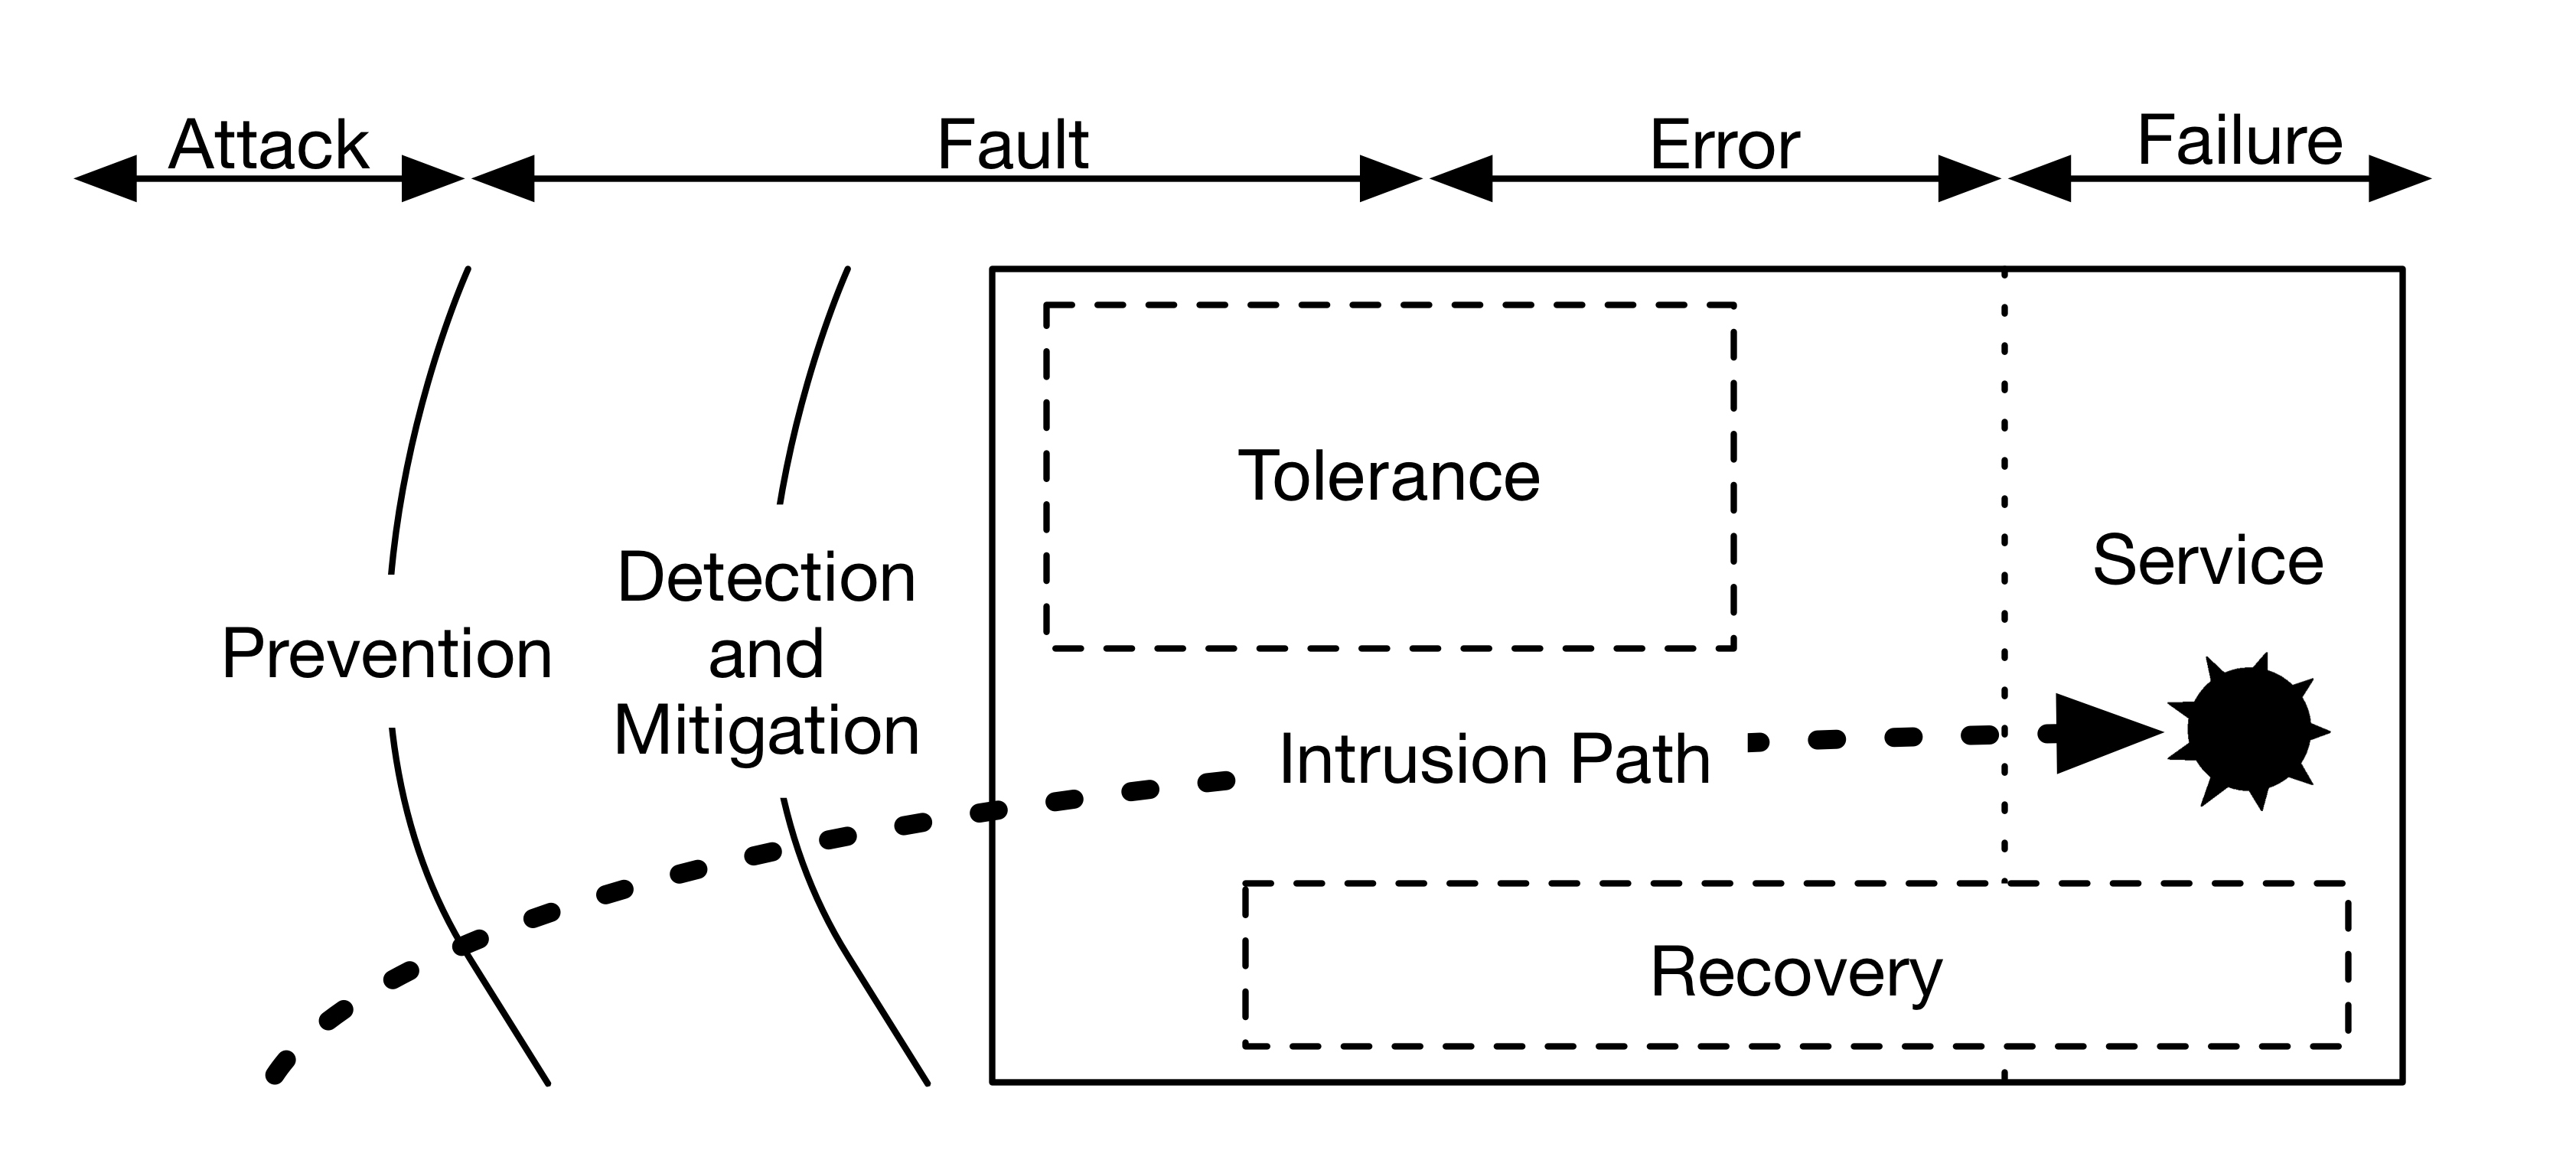
\includegraphics[width=110mm]{images/intrusion}
  \caption{Intrusion path across the system}
  \label{fig:intrusion_path}
\end{figure}

%prevention
\emph{Intrusion forecast and prevention} are realized by design and they seek to prevent future attackers from exploiting vulnerabilities. However, preventing intrusions by design is hard. Software has flaws due to its complexity and budget/time constraints \cite{Charette2005,Landwehr1992}. System administrators, as humans, can make security configuration mistakes or users may grant access to attackers \cite{Brown2001}. Moreover attackers can spend years developing new ingenious and unanticipated intrusions having access to what protects the system while the guardians have to predict them. Due to this asymmetry, it is arguably impossible to protect all vulnerabilities by design. Therefore the vulnerabilities of prevention mechanisms can be exploited successfully leading to an intrusion. A vast number of vulnerabilities and attacks are listed for instance in the National Vulnerability Database \cite{nistNVD}.\\

\emph{Intrusion detection and mitigation} mechanisms monitor the system to detect suspicious actions that may be connected with an intrusion. However, intrusion detection systems turn the system attack-aware but not attack-resilient, that is, they cannot maintain the integrity and availability of the system in face of attacks \cite{Ammann2002}. Intrusion detection systems may not detect unknown vulnerabilities. More, attackers may use encrypted actions or use legitimate requests.\\

%Intrusion Tolerance
\emph{Intrusion tolerance} is the last line of defense against attacks before the system failure occurs (Fig. \ref{fig:intrusion_path}). Intrusion tolerance is the ability of a system to keep providing a, possibly degraded but adequate, service during and after an intrusion \cite{Stavridou2001a}. Instead of trying to prevent every single intrusion, these are allowed, but tolerated. The system has mechanisms to prevent the intrusion from generating a system failure \cite{Verissimo2003}. Intrusion tolerance mechanisms hide the errors effects using redundancy mechanisms or using intrusion recovery systems, which detect, process and recover from intrusions.\\

Many intrusion tolerance mechanisms are based on replicating state with Byzantine fault-tolerant protocols \cite{Schneider1990,Castro2002,Veronese2011}. The idea is to ensure that a service remains operational and correct as long as no more than a certain number of replicas are compromised. Replicas can be implemented in different manners to provide diversity, to reduce the risk of common failure modes. In addition, a proactive recovery mechanism can reboot the replicas periodically to rejuvenate and restore their soft-state and security assets, e.g., keys \cite{Candea2001,Castro2002,Sousa2010}. In \emph{disaster recovery} solutions, the state is replicated in remote sites, allowing the recovery from catastrophes that destroy a site \cite{Wood2010}.\\

The above-mentioned replication mechanisms for intrusion tolerance can tolerate some intrusions targeted at design faults (vulnerabilities), as long as diversity is used. However, most of the fault tolerance mechanisms do not prevent accidentally or malicious faults at application level, e.g., using valid user requests. Most of state replication mechanisms facilitate the damage to spread from one site to many sites as they copy data without distinguishing between legitimate and malicious sources. Furthermore, most of proactive recovery techniques rejuvenate only the application soft-state but intrusions can affect its persistent state. Consequently, intrusions may transverse these intrusion tolerance mechanisms and cause a system failure. 


%!TEX encoding = UTF-8 Unicode

\subsection{Intrusion Recovery}
\label{sec:Recovery}

The main focus of this work are intrusion recovery mechanisms which accept intrusions but detect, process and recover from their effects. These mechanisms remove all actions related to the intrusion, their effects on legitimate actions and return the application to a correct state. These mechanisms can be used to tolerate intrusions or to recover from system failures. In order to recover from intrusions and restore a consistent application behavior, the system administrator detects the intrusion, manages the exploited vulnerabilities and removes the intrusion effects. This process should change the application state to an intrusion-free state.\\

%Detection
The first phase of intrusion recovery, out of the scope of this work, concerns the intrusion detection. Automated intrusion detection systems (IDS) are used to detect intrusions or suspicious behaviors. This phase may need human intervention to prevent false positives, which trigger recovery mechanisms and can result in legitimate data losses. Thus the detection phase can be a significant delay. The detection delay should be minimized because intrusion effects spread in the meantime between intrusion achievement and detection. More, intrusion recovery services should provide tools to help administrators to review the application behavior and determine which weaknesses were exploited. \\

%Correction: Vulnerability repair
The second phase, also out of the scope of this work, is vulnerability management. Vulnerabilities are identified, classified and mitigated after their detection by a group of persons which the NIST names as the patch and vulnerability group \cite{Mell2005}. Vulnerabilities are fixed by configuration adjustments or applying a security software patch, i.e., by inserting a piece of code developed to address a specific problem in an existing piece of software. \\

%Eliminar os efeitos: dependence ficheiros afectados, etc
%- dizer o que o sistema nao faz: lidar com violacoes da confidencialidade
%- dizer que o sistema tambem nao tem que ver com availability, mas que procuramos que o proprio sistema ao recuperar o estado nao tenha impacto na availability
The third phase, and the one that this work is about, consists in removing the intrusion effects. Intrusions affect the application integrity, confidentiality and/or availability. To recover from availability or confidentiality violations is out of the scope of this document. However, we argue that the design of the applications should encompass cryptography techniques which may reduce data relevance and protect the data secrecy \cite{Maheshwari2000}.

Intrusion removal processes recover from integrity violations recreating an intrusion-free state. Due to the fact that the system availability is result of the integrity of each system component \cite{Wang2007}, these processes contribute to recover the system availability. More, the removal processes should not reduce the system availability. We argue that intrusion recovery services should avoid the system downtime and support the execution of recovery processes in background without externalization to users. Intrusion recovery mechanisms can accomplish some of the goals of intrusion tolerance if they keep providing a, possibly degraded but adequate, service during and after an intrusion recovery.

The following sections explain distinct recover processes where the application integrity is restored by determining the effects of the detected intrusion actions, reverting them and recreating a correct state. 
%!TEX encoding = UTF-8 Unicode
\subsection{Formalization of the Recovery Process}
\label{subSec:RecoveryModels}
As discussed in previous section, intrusion recovery services detect the intrusion effects, revert them and restore the application to a correct state. Here we explain this process by formally modeling the application as a sequence of actions and outline the distinct approaches to perform intrusion recovery. \\ 

An application execution is modeled as a set of actions $A$ and a set of objects $D$. Actions are described by a type (read, write, others more complex), the value(s) read/written, and a timestamp (which defines the order of the actions). Each object has a state or value and a set of operations that can modify it. We specify $A_{intrusion}$ as the subsequence of actions of $A$ whereby the attacker compromises the application during the intrusion, $A_{after}$ as the subsequence of actions that begins after the intrusion begin (including the first action of the intrusion) and $A_{legal}$ as the subsequence of legitimate actions in $A$. Notice that $A_{legal} = A - A_{intrusion}$. 

A recovery service aims to set the state of a service to $D_{recovered}$ at the end of the recovery process. The set $D_{recovered}$ shall be composed of objects as if their state was defined exclusively by a set of legitimate actions $A_{recovered}$. The objects of the subset $D_{recovered}$ represent a new \textit{intrusion-free} and \textit{consistent state}. A state is consistent if it is valid according to the application specification. A state is intrusion-free if it is created only by legitimate actions. If the application respects the specification (correctness), then changing from $D$ to $D_{recovered}$ performs service restoration \cite{Aviz}, i.e., restores the application service to a correct behavior.

A basic recovery service, like a full-backup mechanism, tries to obtain, after the recovery, the subset of object values $D_{recovered}$ written before the intrusion, which do not include the attacker actions, i.e., $D_{recovered} = D - D_{after} : D_{recovered} \cap D_{intrusion} = \emptyset$.

We define the set of \textit{tainted} actions, $A_{tainted}$, and the set of tainted objects, $D_{tainted}$, at a certain instant in the following way: if an action belongs to $A_{intrusion}$, then it belows to $A_{tainted}$; if an object belongs to $D_{intrusion}$ then it belongs to $D_{tainted}$; if an action in $A_{legal}$ reads an object in $D_{tainted}$, then that action belongs to $A_{tainted}$; if an action in $A_{tainted}$ writes an object value in $D_{legal}$, then that object belongs to $D_{tainted}$. Therefore, $A_{tainted}$ includes $A_{intrusion}$ but typically also actions from $A_{legal}$ that were corrupted by corrupted state. Also, $D_{tainted}$ includes $D_{intrusion}$ but typically also objects from $D_{legal}$ that were corrupted by corrupted state. Then, the set of object values written only by non-malicious actions is not the same as the set of objects obtained after removing the objects written by malicious or tainted actions, i.e., $D_{legal}$ written by $A \cap A_{intrusion} = \emptyset$ is not equal to $D_{legal}$ written by $D-D_{intrusion}$ or $D_{legal}$ written by $D-D_{tainted}$. In other words, to remove the objects written by intrusions and tainted actions is necessary but not enough to obtain the values of the set of objects that would be produced only by legitimate actions.

Some intrusion recovery systems \cite{taser,itdb,phoenix} attempt to obtain $D_{recovered}$ where the values of the objects of $D_{tainted}$ are removed from the current state $D$. To do so, the value of each object in $D_{tainted}$ is replaced by a previous value. These systems keep the objects written by legitimate actions, $D_{legal}$, unmodified. \\


Consider an hypothetical application execution at a certain point in time, after the intrusion, where $A$ is replaced by the set $A_{recovered} = A - A_{intrusion} = A_{legal}$, i.e., where the intrusion actions $A_{intrusion}$ are not executed. We would have in this application: $A \cap A_{intrusion} = \emptyset \implies D_{intrusion} = \emptyset, A_{tainted} = \emptyset \implies D_{tainted} = \emptyset$. In other words, if the malicious action are removed, the state, $D$, does not have the objects written by $A_{intrusion}$. For this reason, the sequence of tainted actions $A_{tainted}$ is empty. The set of tainted actions in the real application execution, which includes $A_{intrusion}$, would read different values and have a different execution if $A_{intrusion}$ would be empty. Therefore, if $A_{intrusion}$ and $D_{intrusion}$ are removed, then $A_{tainted}$ should be \emph{replayed} because the actions of $A_{tainted}$ are not contaminated by malicious data during their re-execution. The replay process restores the application to a correct state $D_{recovered}$, which is intrusion-free.\\

The sequence of actions, $A_{before}$, performed before the intrusion, i.e., $A_{before} = A - A_{after}$, can be extensive. Each action takes a variable but not null time to perform. Therefore, to replay $A_{recovered} : A_{before} \subseteq A_{recovered} $ may takes an excessive amount of time. We define the subsets $D_{snapshot}(t)$ and $A_{snapshot}(t) : A_{snapshot} \subseteq A$ as the subsets of object values and actions executed before the begin of a snapshot operation at instant \textit{t}. The snapshot operation copies the value of the object immediately or on the next write operation. If the attack is subsequent to $t$, then $A_{after} \cap A_{snapshot} = \emptyset \implies (A_{intrusion} \cup A_{tainted}) \cap A_{snapshot}(t) = \emptyset$, i.e., the snapshot is not affected by intrusion. For that reason, the service can replay only $A-A_{snapshot}-A_{intrusion}$ using the object set $D_{snapshot}$ as base. 


The works explained in the following sections define two distinct approaches to update the set of object $D$ to $D_{recovered}$ because of changes in the execution of $A_{tainted}$: \textit{rewind} and \textit{selective replay}. The selective replay approach loads only the previous versions of the tainted objects, $D_{tainted}$, and replays only the legitimate operations, which were tainted, $A_{tainted} \notin A_{intrusion}$, to update the objects in $D$. The $D_{legal} \notin D_{tainted}$ remain untouched. The alternative approach, rewind \cite{Brownc}, designates a process that loads a system wide snapshot previous to the intrusion moment and replays every action in $A-A_{snapshot}-A_{intrusion}$. However, this process can take a long time. \\


 A \textit{version} is a snapshot of a single object value before the instant $t$. They can be recorded with the sequence of actions that read or write them before the instant $t$. We define a \textit{compensating} action as an action that reverts the effects of a original action, for instance writing a previous value. A compensation process can obtain a previous snapshot or version. For this propose, we define the sequence $A_{compensation}(t)$ as the compensation of $A_{posteriori}(t)$, the sequence of actions after instant $t$. The compensation process applies the sequence of compensating actions $A_{compensation}(t)$ on the current version of the objects, in reverse order, to obtain a previous snapshot or version.\\

Recovery services have two distinct phases: \textit{record phase} and \textit{recovery phase}. The record phase is the service usual state where the application is running and the service records the application actions. In order to perform replay, the application actions do not need to be idempotent but their re-execution must be deterministic. The record phase should record the actions input and the value of every non-deterministic behavior to turn their re-execution into a deterministic process. The recovery phase can have three phases: determine the affected actions and/or objects, remove these effects and replay the necessary actions to recover a consistent state, as already explained in Section \ref{sec:Recovery}. The recovery services that support \textit{runtime recovery} do not require application downtime because the record and recovery phases can occur simultaneously.\\


Most of intrusion recovery services record the actions and track the objects accessed by each of them. Since the actions read and write objects from a shared set of object values $D$, we can establish dependencies between actions. Dependencies can be visualized as an \textit{action dependency graph} or an \textit{object dependency graph}. The nodes of an action dependency graph represent actions and the edges indicate dependencies though shared objects. The object dependency graph establishes dependencies between objects through actions. Dependency graphs are used to order the re-execution of actions \cite{undoForOperators}, get the sequence of actions affected by an object value change \cite{warp}, get the sequence of actions tainted by an intrusion \cite{Akkus2010} or resolve the set of objects and actions that caused the intrusion using a set of known tainted objects \cite{backtracker}. 

A \textit{taint algorithm} aims to define the tainted objects $D_{tainted}$ from a source sequence of malicious actions $A_{intrusion}$ or objects $D_{intrusion}$ using the dependency graph. The \textit{taint propagation via replay} \cite{retro} algorithm begins with the set of $D_{tainted}$ determined by the base taint algorithm and expands the set $D_{tainted}$. It restores the values of $D_{intrusion} \cup D_{tainted}$ and replays only the legal actions that output $D_{intrusion} \cup D_{tainted}$ during the original execution. Then it replays the actions dependent from $D_{intrusion} \cup D_{tainted}$, updating their output objects. While the forward actions have different input, they are also replayed and their outputs are updated.\\

Dependencies are established during the record phase or at recovery time using object and action records. The level of abstraction influences the record technique and the dependency extraction method. The abstraction level outlines the recoverable attacks. In the next paragraphs, we explain the relevant works at abstraction levels where services deployed in PaaS are attacked: operating system, database and application.\\



%!TEX encoding = UTF-8 Unicode
%
% Estrutura da analise: 
%     - Summary
%     - How records? How determines the affected?
%     - How removes the effects?
%     - Does it perform replay? How? Of What?
%     - Extra characteristics
%     - Analyze/comments
%
\subsection{Recovery at Operating System Level}
\label{sec:recovery_os}

In this section, we present the main intrusion recovery proposals for operating systems. First, we present the proposal that introduced the main dependencies for operating systems. Then, we present two intrusion recovery systems that use dependency rules and tainting propagation via replay, respectively. Finally, we present proposals to recover from intrusions in computing clusters, virtual machines and network file systems.\\

\textbf{BackTracker \cite{backtracker}:} Backtracker proposes a tainting algorithm to track intrusions. It does not perform any proactive task to remove or recover from intrusions but provides a set of rules for intrusion recovery in operating systems.

Backtracker proposes a tainting algorithm that does tainting analysis offline, after attack detection, as follows. First a graph is initialized with an initial set of compromised processes or files, $D_{tainted}$, identified by the administrator. Then, Backtracker reads the log of system calls from the most recent entry until the intrusion moment. For each process, if it depends on a file or process currently present in the graph then the remaining objects dependent from the process are also added to the graph. The result is a dependency graph (Fig. \ref{fig:graph}) with the objects, including $D_{intrusion}$, which the compromised objects depend from. The following dependency rules establish the graph edges:

\begin{itemize}
  \item \textit{Dependencies process-process:}
  \begin{itemize}
    \item \textit{Process depends on its parent process}: Processes forked from tainted parents are tainted.
    \item \textit{Thread depends on other threads}: Clone system calls to create new threads establish bi-directional dependences since threads share the same address space. Algorithms to taint memory addresses \cite{bezoar} have a significant overhead. Signaling communication between processes also establish dependencies.
  \end{itemize}
  \item \textit{Dependencies process-file:}
  \begin{itemize}
    \item \textit{File depends on Process:} If the process writes the file.
    \item \textit{Process depends on File:} If the process reads the file. 
  \end{itemize}
  
  \item \textit{Dependencies process-filename:}
  \begin{itemize}
    \item \textit{Process depends on filename:} If the process issues any system call that includes the filename, e.g., open, create, link, mkdir, rename, stat, chmod. The process is also dependent of all parent directories of file.
    \item \textit{Filename depends on process:} If any system call modifies the filename, e.g., create, link, unlink, rename.
    \item \textit{Process depends on directory:} If the process reads one directory then it depends on every all filenames on directory.
  \end{itemize}
\end{itemize}

\begin{figure}
  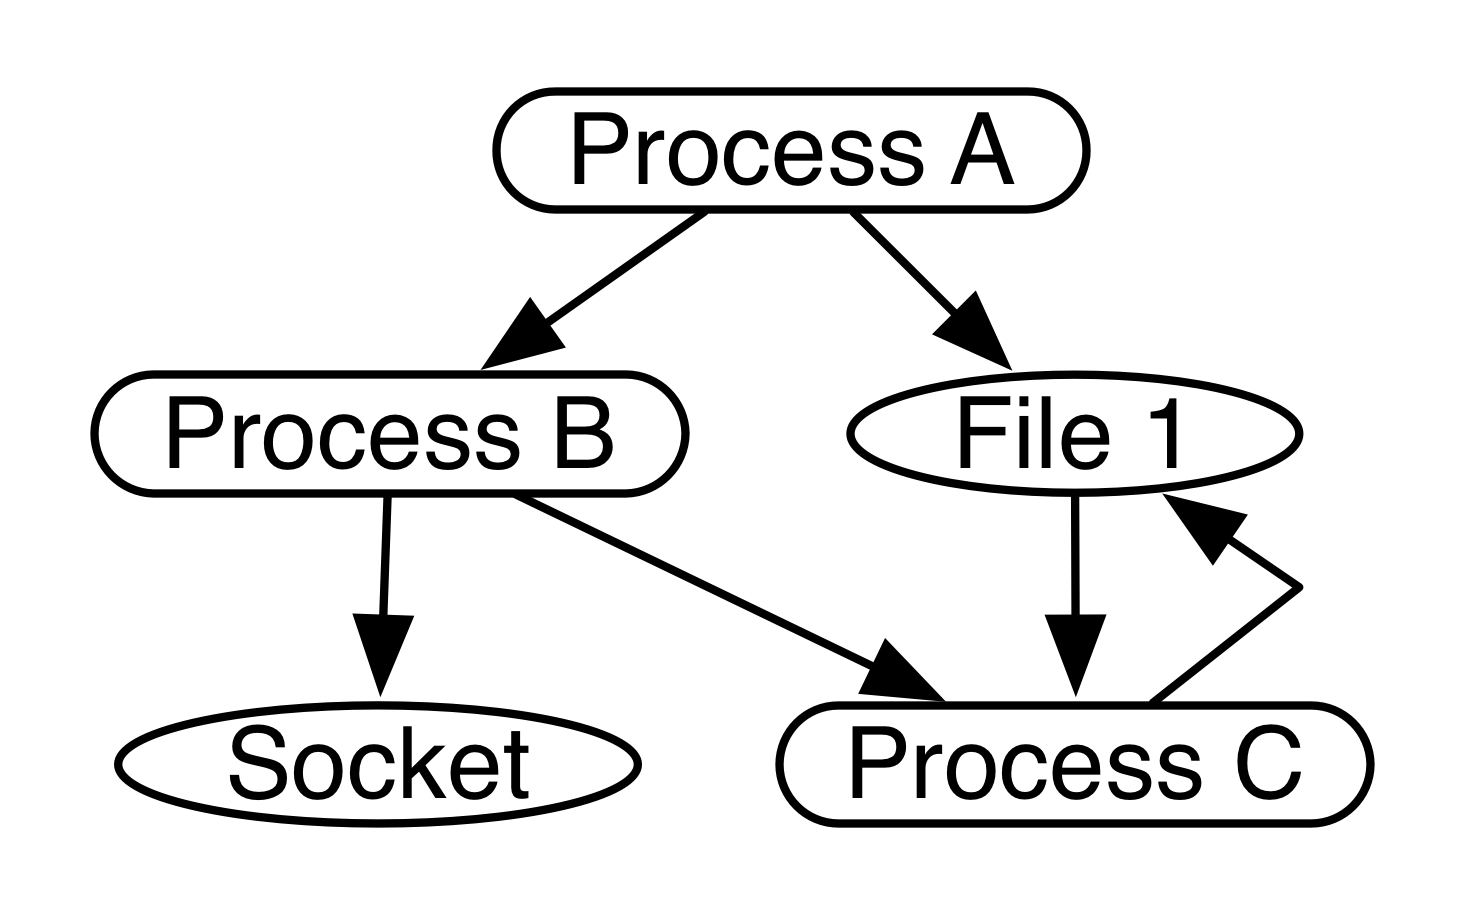
\includegraphics[height=30mm]{images/depGraph}
  \centering
  \caption{Dependency graph generated by BackTracker}
  \label{fig:graph}
\end{figure}

Objects shared between many processes, e.g., \textit{/tmp/} or \textit{/var/run/utmp} are likely to produce false dependencies leading to false positives. Therefore, Backtracker proposes a \textit{white-list} filter that ignores common shared files. However, this technique relies in the administrator knowledge. More, it generates false negatives because it allows the attackers to hide their actions in objects that belong to the white-list. \\


\textbf{Taser \cite{taser}:} Taser removes the intrusion effects from the file system used by the operating system. To do that, it loads a previous version of each tainted file, $D_{tainted}$, from a file-system snapshot, $D_{snapshot}(t)$. Then, to recover the tainted objects, it replays the legitimate modification actions of each tainted object since the snapshot instant $t$.

%record phase
Taser relies on Forensix \cite{forensix} to audit the system actions during the record phase. Forensix logs the names and arguments of every system call related to process management, file system operations and networking. In order to determine the intrusion effects, Taser builds a \textit{object dependency graph} using a set of rules similar to the rules of Backtracker \cite{backtracker}. The object definition encompass files, sockets and processes. Since these rules result in a large number of false dependencies, which mark legitimate objects as \textit{tainted}, Taser provides not only a white list mechanism but also establishes optimistic policies that ignore some dependencies. However, attackers can leverage these optimistic policies to penetrate the operating system.

%How it determines the affected elements?
The recovery phase is started with a set of tainted objects provided by an administrator or an IDS. The provided set of objects can either be the source or the result of an attack. In the latter case, Taser, like Backtracker \cite{backtracker}, transverses the dependency graph in reverse causality order to identify the set of attack source objects, $D_{intrusion}$, which compromised the provided objects. After, at \textit{propagation phase}, Taser transverses the dependency graph from the source objects of the attack, $D_{intrusion}$, to the current moment, adding all tainted objects to the set $D_{tainted}$.

%how it removes
Taser removes the intrusion effects loading a previous version of the tainted objects from a file-system snapshot, $D_{snapshot}(t)$. Then, to recover a coherent state, Taser performs \textit{selective replay}, i.e., it replays, sequentially, the legitimate write operations of the tainted files since the snapshot. Non-tainted files remain unchanged. Since Taser does not checkpoint the state of processes nether the input of each system call, the system must be restarted to remove the current non-persistent states and processes must be replayed from the beginning to load their non-persistent state and perform their system calls with the correct state. This issue has a significant overhead specially for long-run processes as web servers.

 
%does it replays? analyze
Taser does not update the objects originally dependent from tainted objects. In other words, the replay process only recovers a consistent state for the originally tainted objects. Therefore, Taser ignores the set of actions that read the modified version of the tainted files and have a different execution and output. This problem is addressed in \cite{Shafique2006}. More, Taser uses rules to determine the affected files and remove their effects, so it can mistakenly mark legitimate operations as tainted and induce to legitimate data losses.\\



\textbf{RETRO \cite{retro}:} RETRO provides the capability of removing files affected by a set of identified attacking actions. It restores the corrupted files to a previously version using a file system snapshot and then performs selective replay using \textit{taint propagation via replay}. 

%Record Phase:
During the record phase, the kernel module of RETRO creates periodic snapshots of the file system. RETRO logs the input and the output objects of each system call and their associated process. The object definition encompasses not only files and directories but also TCP sessions and the operating system console (tty). The dependencies are established per system call instead of per process. Therefore, the graph is finer-grained than the graph of Backtracker \cite{backtracker} and reduces the number of false positives.

%remove
During the recovery phase, RETRO requires the administrator to identify $A_{intrusion}$, processes, system calls or $D_{intrusion}$ objects which caused the intrusion. First, it removes the malicious system calls from the graph. Then it performs \textit{taint propagation via replay}. To do so, it loads a previous version, from a snapshot, of the objects in $D_{intrusion}$. Then, the system calls, which are dependent from the restored objects, are replayed and their output objects are updated. The forward system calls, which depend from the updated objects, are also replayed while their inputs are different from the original execution. The propagation is done thought the output of system calls with different execution. The recovery process terminates when propagation stops. Since RETRO records the system call input, it can replay processes with system call granularity instead of process granularity, so the replay process may stop earlier. However, this mechanisms forces that the process re-execution has the same sequence of system calls as its original execution. Therefore, the process source code nether its sequence of actions can not change. 

%external dependencies
Since RETRO replays the processes, the external state may change. External changes are manifested through operating system console and network objects. RETRO emails the administrator with the textual difference between the original and recovery outputs. Later work of the same authors, \textit{Dare} \cite{dare}, extends RETRO to recover from intrusions in distributed systems. It adds the dependencies through sockets. The machines involved in a network session add socket objects to the dependency graph. Network protocol, source and destination IP and ports and one ID, which are exchanged in every package during the connection, globally identify each socket object. The recovery phase in Dare is similar RETRO except on network system calls handlers. Compromised network sessions must be replayed since their input depends on destination server. Therefore, prior to invoke the system call for network session establishment, Dare invokes a remote method at receiver Dare daemon to rollback the network session. The receiver rollback the dependent objects to the version before session establishment and replays their dependencies. The remote method response includes the re-execution output. The local system updates the system call output. The re-execution is propagated if this output is different. 

%Analyse
The efficiency of RETRO comes from avoiding to replay the actions if their input remains equal. However, the invoked system call must remain the same. Therefore, RETRO does not support a distinct process execution. RETRO requires human intervention to solve external inconsistencies. Dare solves it but it is limited to clusters where every operating system runs a Dare and RETRO daemon. RETRO can not recover from an intrusion whose log files have been garbage collected or deleted. Dare supports distributed re-execution but, as RETRO, the affected machines must be offline because its propagation algorithm shutdown the service during the repair phase. \\



\textbf{Bezoar \cite{bezoar}:} Bezoar proposes a rewind based approach to recover from attacks coming from the network in virtual machines (VM). The snapshot is performed by VM forking using copy-on-write. This snapshot technique encompasses the entire system: processes and kernel spaces, resources, file system, virtual memory, CPU registers, virtual hard disk and memory of all virtual external devices. Bezoar tracks how the data from network connections propagates in memory. During the recovery phase, the administrator identifies the network connections used by the attackers. Bezoar removes the intrusion effects using rewind. It loads a previous VM snapshot and it replays the system execution ignoring all network packets from the identified malicious sources. 

The recovery process using rewind is longer than RETRO or Taser because all external requests are replayed but supports distinct process execution. Bezoar requires system outage during the replay phase and does not provide any external consistency warranties.\\


\textbf{Repairable File System (RFS) \cite{rfs}:} RFS is designed to recover compromised network file systems. The novelty in RFS comparing with the previously introduced systems is its client-server architecture. RFS includes a client and a server module for a network file system (NFS).

The client module tracks the system calls using ExecRecorder \cite{Oliveira2006} and establishes the dependence between processes and NFS requests. Every request to the NFS server is marked with a request ID and the client ID. At server side, the request interceptor logs all requests sent by clients to update files. Requests are ordered in per-filename queues. They are processed locally and write operations are mirrored to external server asynchronously after reply. The external server keeps all file versions. 

During the recovery phase, the server defines the contaminated processes using the client logs. A process is contaminated if it matches a set of rules similar to Backtracker \cite{backtracker}. RFS adds the concept of contaminated file and contaminated file block. If a file is contaminated, all its blocks are contaminated. The reverse is not true, i.e., processes remains non-contaminated if they read a correct block from a contaminated file. RFS uses the version server to rollback only the affected files. \\



\textbf{Summary:} Dependencies at the operating system level are established by rules based on BackTracker \cite{backtracker}. These rules are vulnerable to false positives and false negatives. While Taser \cite{taser} and RFS \cite{rfs} recover from intrusions removing the effects only in corrupted files, RETRO \cite{retro} removes the values written by $A_{intrusion}$ and replays the forward system calls while their input changes. If $A_{intrusion}$ is identified properly, then RETRO does not have false positives.

The operating system level services are vulnerable to attacks inside kernel because they only audit the system calls. Attackers can compromise the recovery system because the log daemons are installed in the machine where attacks are performed. The recovery guarantees are limited by the system administrator capability to detect the attack and pinpoint the intrusion source. Administrators must avoid false positives to prevent legitimate data losses. However, remove false dependencies can take a while because the low abstraction level creates bigger dependency graphs and logs.




%!TEX encoding = UTF-8 Unicode
\subsection{Recovery at Database Level}
\label{sec:recovery_database}




A vast number of database management systems (DBMS) support recovery by loading a snapshot (or full-backup) of the database, possibly patched with blocks of data modified since the snapshot was taken. However, this approach does not distinguish between malicious and legitimate requests. The recovery approach we are interested in the document is applied to databases similarly to what was seen in Section \ref{sec:recovery_os} for operating systems. While the operating system dependencies are established by the system calls, the database dependencies are established by transactions. First, we define the main dependencies in the database systems. These rules are used by most of the recovery services for databases and applications (Section \ref{sec:recApp}).\\

Compromised transactions are determined from an initial set of bad transactions using read and write rules. ``Transaction $ T_j$ is dependent upon transaction $ T_i$ if there is a data item $x$ such that $T_j$ reads $x$" \cite{Ammann2002} and $T_i$ performs the latest update $x$. Transaction dependency is transitive. ``A good transaction $G_i$ is suspected if some bad transaction $B_i$ affects $G_i$. A data item $x$ is compromised if $x$ is written by any bad or suspect transaction" \cite{Ammann2002}. This dependency chain is broken if a transaction performs a blind write, i.e., the transaction writes an item without read it first.

However, legitimate transactions can have different outputs even when their original execution were not tainted. For example, a malicious transaction can remove a data entry which the following transactions would read and then write other data entries. Since user mistakes are often deletes due to wrong query arguments, this is a relevant issue. Xie \textit{et al.} \cite{Xie2008} propose to track the transaction that deleted the data entries keeping a copy of deleted data entries in a separated database table. To add the dependencies from the deleted data items, the SQL statement is performed in the original and delete tracking tables. 

The dependency rules require to extract the read and the write set of each transaction, i.e., the set of data entries that each transaction read or modifies. The following proposals use different methods to extract these sets and restore the tainted data entries.\\


\textbf{ITDB \cite{itdb,Ammann2002,Wang2007}:} Intrusion Tolerant Database (ITDB) performs intrusion recovery in databases using compensating and supports \textit{runtime recovery}, i.e., the database service remains available during the recovery process. ITDB uses the generic set of dependency rules mentioned in the beginning of Section \ref{sec:recovery_database} and extracts the read and write set parsing the SQL statements.

During the record phase, ITDB audits the read and write sets of each transaction. Most relational DBMS only keep write logs. Therefore, Liu \textit{et al}. \cite{itdb} propose a pre-defined per-transaction type template to extract the read set of parsed SQL statements. This approach is application dependent since updates in application queries require updates in their templates. 

%algoritmo de recovery
At recovery phase, ITDB initiates a set $D_{tainted}$ with the intrusion source data items. Then, it reads the log of read and write sets of each transaction from the intrusion moment to the present. For each transactions, ITDB keeps the write set until the transaction commits or aborts; if the transaction commits after reading some data item that belongs to $D_{tainted}$, ITDB adds the data items in the transaction write set to $D_{tainted}$ and the transaction must be compensated. The compensating of a transaction reverts the effects of the original transaction. It performs the inverse modification of the original transaction to restore the previous values. Repaired entries in $D_{tainted}$ are tracked to prevent compensating of later transactions from restore a repaired data entry to its version after the attack. After this process, the latest legitimate value of $D_{tainted}$ entries is recovered.

%extras
If the intrusion propagation is faster than the recovery process then the recovery phase is endless because the damage will spread through new transactions. To prevent damage spreading, ITDB blocks the read accesses to the data entries in $D_{tainted}$. Since identification of $D_{tainted}$ requires log analysis, Liu \textit{et al.} propose a \textit{multi-phase damage container} technique to avoid damage spread through new requests during the recovery phase. This damage containing approach denies the read access to the data items were written after the intrusion. Then, during the recovery phase, it releases the data entries that were mistakenly contained. This approach speeds-up the recovery phase and confines the damaged data items. More, it supports \emph{runtime recovery}. However it decreases the system availability during the recovery period and degrades the performance.

An alternative approach concerns the throughput asymmetry between the recovery and the user flows. The asymmetry can be neutralized if the repair request priority is increased. Then, the availability is not compromised anymore but users may read tainted data and propagate the damage slower. 

The ITDB architecture includes an intrusion detection system. The IDS is application aware and acts at transaction level. Liu \textit{et al.} propose isolation in terms of users: when a suspicious transaction is reported by the IDS, every write operation from the suspicious user is done in isolated tables.

The ITDB does not perform transaction replay during the recovery phase. Therefore, it ignores that legitimate executions can be influenced by the updated values. Liu \textit{et al.} propose a theoretical model \cite{Yu2003} based on possible workflows and versioning. However, predict every possible workflow requires extensive computational and storage resources. \\


\textbf{Phoenix \cite{phoenix}:} Phoenix removes the intrusion effects using a versioned database. While Liu \textit{et al.} \cite{Ammann2002} rely on templates of SQL statements and read the log in recovery time, Phoenix changes the DBMS code to extract read dependencies and proposes a runtime algorithm to check dependencies between transactions.

%Versioning
Phoenix performs every write operation appending a new row to the table. This new row includes an unique transaction id to support the restoration of previous row versions. Phoenix modifies the PostgreSQL DMBS code to intercept read queries during their execution and to extract the transaction id of each accessed row. The logged data is used to update the dependency graph.

%Como funciona
At the recovery process, Phoenix identifies the set of affected transactions, $A_{tainted}$, from a root set of malicious transactions, $A_{intrusion}$, using the dependency graph. Then, it changes these transactions status to \textit{abort} in the PostgreSQL transaction log. Since PostgreSQL, in serializable snapshot isolation mode, exposes only the row version of the latest non-aborted transaction, the row is restored and the effect of tainted transactions are removed.\\


\textbf{Summary:} Recovery systems for relational databases differ on their methods to track the read and write sets and to restore previous values. ITDB is application dependent because it requires pre-defined templates to parse the SQL statements. On the other hand, Phoenix is application independent but DBMS dependent because it modifies the DBMS source code and relies on the usage of serializable snapshot isolation mode. 

ITDB is records the previous versions in contrast to Phoenix which just records the transactions. The first requires more storage capacity to save the versions, the second requires the knowledge of the compensating of each transaction and more computation resources during recovery to revert the tainted transactions.

The data item granularity affects the runtime performance overhead and the accuracy of dependency tracking. Coarser granularity, e.g., row, results in lower performance overhead but a higher probability of false dependence if two transactions read and write different portions of the same data item. Moreover, an attack can compromise just an independent part of the transaction and legitimate data is removed. 
%!TEX encoding = UTF-8 Unicode
\subsection{Recovery at Application Level}
\label{sec:recApp}
Web applications are the main type of application which is deployed in PaaS. These applications are usually composed of a three tier architecture: presentation tier, application-logic tier and data tier. The following works assume the data tier to be a database. 
Previous section works establish the dependencies between transactions using their read and write sets. However, they ignore the dependencies between transactions at application level. For example, an application can read a record A through a transaction 1, compute a new value B, based on A, and write the value B through a transaction 2. The application-logic tier is often state-less, the requests are independent and the database is the only mean of communication between requests (Section \ref{sec:PaaS}).\\ 


\textbf{Data Recovery for Web Applications \cite{Akkus2010}:} Goel \textit{et al.} propose a recovery service that selectively removes intrusion effects from web applications that store their persistent data in a SQL database. Since each user request may involve multiple transactions, it tracks the user, the session, the request and the accessed rows. The proposal uses a tainting algorithm and compensating transactions.

During the record phase, a monitor logs each user request and the database rows and tables read and written by the transactions associated with it. The transactions are stamped with an id that establishes the replay order, since the database uses serializable snapshot isolation.

The recovery phase is as follows. First, the administrator, using the logged data, identifies the malicious requests $A_{intrusion}$. Then, using a dependency graph, it determines the tainted requests. The dependency between transactions is established in a similar manner to the Section \ref{sec:recovery_database} but using table granularity instead of row granularity. Such coarse-grained approach may generate many false dependencies. Therefore Goel \textit{et al.} use \textit{taint propagation via replay}. More, it proposes to modify the PHP-interpreter to reduce the false dependencies between transactions using a variable-level tainting. In other words, variables that read tainted rows or fields are also tainted; rows or fields written by tainted variables are tainted. This process increases the precision of the set of tainted requests. Finally,the compensation transactions of the tainted requests are applied in reverse serialization order on the current state of the database to selectively revert the effects of the database operation issued by the tainted requests.\\ 

\textbf{POIROT \cite{poirot}:} POIROT is a service that, given a patch for a newly discovered security vulnerability in a web application code, helps administrators to detect past intrusion that exploited the vulnerability. POIROT does not recover from intrusions but proposes a tainting algorithm for application code. During the normal execution, every user request and response is stored. The log of each request includes the invoked code blocks. After the attack discover phase, the software is updated to fix its flaws. POIROT identifies the changed code blocks and requests dependent from them during the normal execution. The affected requests are replayed. During the re-execution phase, each function invocation is forked into two threads: the updated e non-updated version \cite{Wang2011}. Functions invocations are executed in parallel and their output are compared. If outputs are similar, only one execution proceeds otherwise the request execution stops since the request was affected by code patch. These concepts are used in Warp \cite{warp}.\\


\textbf{Warp \cite{warp}:} Warp is a patch based intrusion recovery service for single server web applications backed by a relational database. Unlike previous approaches, Warp allows administrators to retroactively apply security updates without tracking down the source of intrusion and supports attacks at user browser level. Warp is based on RETRO \cite{retro} \emph{taint propagation via replay} approach and removes the intrusion effects using a versioned database. The Warp prototype uses PHP and PostgreSQL. 

%normal
During the normal execution, Warp uses a client browser extension to record all JavaScript events that occur during the visit of each page. For each event, Warp records the event parameters, including the target DOM element. HTTP requests are stamped with a client ID and a visit ID to track dependencies between requests at browser level. On server side, Warp records every requests received and forwards the request to the PHP application. Since Warp uses PHP, an interpreted language, it records which files were used during the original request execution and records the non-deterministic functions. Warp stores the database queries input/output and tracks the accessed table partitions using a SQL statement parser. To conclude, the HTTP response is logged and packed with all execution records.

Warp includes a time-travel versioned relational database. Each row is identified using a row ID and includes a \textit{start time} and \textit{end time} timestamp columns that establish the row validity period. Warp reverts the intrusion effects, in a specific row, loading one of its previous versions. Warp supports concurrent repair using more two integer columns to define the begin and end of each \textit{repair generation}. At repair phase, the current repair generation ID is incremented to fork the database. User requests are performed in the current generation while recovery requests are perform in the next generation. After replaying the requests retrieved until the begin of the repairing process, the server stops and applies the remain requests.

%Como determina
During the repair phase, the administrator updates the application software to fix its flaws. Then, Warp determines the requests used the modified source code files \cite{poirot,Wang2011}. These requests are the root cause of changes during the re-execution. To update the database and reflect the patch, each user request is replay using a server-side browser and taint propagation via replay. The modified PHP interpreter intercepts non-deterministic function calls during the replay and returns the original logged value. Also, database read queries are replayed only if the set of affected rows is different or its content was modified. Write queries are replayed loading a previous version of the rows and replaying the SQL statement. Each row, which has a different result after re-execution, is now tainted and all requests that read the row are also marked to replay in the browser. Finally, the HTTP response is compared with original. If responses are different, the following dependent user interactions are replayed in the server side browser.

%Extra
The server-side browser may fail to replay the original user request. The request may depend from a reverted action of the attacker. These conflict cases are queued and handled by users later. 

%Comments 
Warp rewrites the SQL statements, which are used by the application to perform write operations in the database, adding four extra columns per table: start/end timestamp and start/end generation. However, these columns may be a considerable storage overhead. It also depends from a client browser extension to log and modify every request. Warp is designed for single machine applications: it does not support application deployed in multiple servers or distributed databases since versions are timestamp based. \\


\textbf{Aire \cite{aire}:} Aire is an intrusion recovery service for loosely coupled web services. It extends the concept of local recovery in Warp \cite{warp} tracking attacks across services. While Dare \cite{dare} aims to recover a server cluster synchronously using RETRO \cite{retro} in each node operating system, Aire performs recovery in asynchronous third-party services using Warp \cite{warp}. 

Aire prevents the recovery process from locking due to remote servers downtime. To achieve this goal, the pendent repair requests are queued until the remote server is recovered. Since clients may see a partial repaired state, Aire proposes a model based on eventual consistency \cite{Decandia2007,Vogels2009}. The model allows clients to observe the result of update operations in different orders or delayed during a period called \textit{inconsistency window}, i.e., until the remote server recovers. Aire considers the repair process as a concurrent client. To repair key-value database entries, Aire creates a new branch \cite{git} and re-applies legitimate changes. At end of local repair, Aire moves the current branch pointer to the repaired branch.

Like Warp \cite{warp}, during the normal execution, Aire records the service requests, responses and database accesses. Requests and responses exchanged between web-services, which support Aire, are identified using an unique ID to establish the dependencies.


The recovery phase is as follows. First, the administrator identifies the corrupted requests. The administrator can create, delete or replace a previous request or change a response to remove the intrusion actions. Second, Aire creates a new branch which will contain the set of changes. Third, Aire does a local repair of the application in a similar manner to Warp \cite{warp}. In contrast to Warp \cite{warp}, starts the recovery process in remote servers if at least one of the requests or responses sent previously is modified. To do so, Aire sends a request to the source or destination of the modified message. If the remote server is offline, the repair request is queued to be sent later. As repair messages propagate between the servers to start successive repairing actions, the global state of the system is repaired. However, clients may see an inconsistent state during this process. Therefore, Aire applications must support eventual consistency.  

The Aire approach using eventual consistency requires the developer to concern the conflict resolution. Moreover, Aire recovers third-party web-services which must have an Aire daemon. Aire requires the administrator to pinpoint the corrupted requests. Finally, Aire, as Dare \cite{dare}, requires application downtime during the recovery process.\\



\textbf{Undo for Operators \cite{undoForOperators}: }Undo for Operators allows the system administrators to recover from their mistakes, software problems or data corruption in email services with file system storage. The design is base on ``Three R's: Rewind, Repair and Replay" \cite{Brownc} where operator loads a system-wide snapshot previous to the intrusion, repairs the software flaws and replays the user-level requests to recover a correct application state. In contrast to the selective replay approach, where only the tainted entries are reverted, the rewind reverts all database entries. On one hand, it requires to replay more requests. On the other hand, it does not require to determine which data entries are tainted because every entry is reverted.

Undo for Operators proposes a proxy interposed between the application and its users. The proxy intercepts application requests. Since rquests most be ordered to replay, Undo for Operators defines the concept of \textit{verb}. Each protocol operation has its own \textit{verb} class. A verb object encapsulates a single interaction (request/response) of the user and exposes an interface to establish the order between requests and their dependencies. However, the proposed architecture is protocol dependent. The proxy implementation only supports IMAP and SMTP. A new protocol requires a new set of verbs. 

During the normal execution, user requests are encapsulated into verbs and sent to a remote machine: the \emph{undo manager}. The undo manager uses the interface of verbs to define its dependency, i.e., if it can be executed in parallel or must have a causal order with other request. The dependency is established per verb type depending from the operation and its arguments. Thus, the dependency mechanism is application dependent. For example, send email operations (SMTP protocol) are commutable and independent because the email delivery does not have ordering guaranties. On the other hand, the order of delete (expunge) and list (fetch) operations in the same folder is relevant and they are not independent. If two verbs are dependent, the second is delayed upon the first is processed. This method establishes a serialization ordering but it can create a significant performance overhead on concurrently arriving interactions and requires protocol knowledge.

The recovery phase strategy is as follows. First the operator determines the corrupted verbs and fixes their order adding, deleting or changing verbs. Second, the application is \textit{rewind}, i.e., a system-wide snapshot is loaded to remove any corrupted data. Third, the operator patch the software flaws of the application. Finally, all legitimate requests started after the intrusion, $A_{legitimate}$, are re-sent by the proxy to rebuild the application state. 

External inconsistencies may come out when the requests are replayed. These inconsistencies are detected comparing the re-execution and the original responses. Different responses trigger a compensating action defined per verb to keep an external consistent state. Again, these actions are application dependent.

During the recovery process, Undo for Operators replaces the current system state by a system wide snapshot. Consequently, it does not support runtime recovery. Moreover, it relies on protocol knowledge to establish dependencies, compensating actions and to sort the requests during the normal execution and recovery phase. Therefore, any protocol change requires to modify the supported verbs. Intrusions can use corrupted requests which are not defined as verb classes and cause a system fail.\\


\textbf{Summary:} Goel \textit{et al.} and Warp \cite{warp} establish dependencies using the request read/write set of the database and use taint via replay. Undo for Operators \cite{undoForOperators} establishes dependencies using the knowledge of the operations protocol. Unlike Goel \textit{et al.}, Warp \cite{warp} and Undo for Operators \cite{undoForOperators} support application repair. Warp tracks the requests affected by the modified file. Undo for Operators replays every request using its proxy. While Goel \textit{et al.} ignores external consistence, Warp \cite{warp} detects inconsistencies in responses and replays the user interaction in a browser and Undo for Operators uses compensating actions based on protocol-specific knowledge.

The approaches to remove the intrusion effects are also distinct. Goel \textit{et al.} uses compensating transactions to create a system wide snapshot, Undo for Operators loads a previous snapshot and Warp keeps the versions of each data entry. If the tainted request are few, then Goel \textit{et al.} and Warp have a significant advantage because they replay only the tainted requests. On the other hand, Undo for Operators requires less storage than the remaining options. More, the knowledge of inverse transaction is required to create the compensation of transactions. \\
\subsection{Evaluation of Technologies}
\label{sec:Discuss}
The previous subsections describe various services that use different approaches to recover from intrusions. The level of abstraction outlines the recorded elements. Intrusion recovery services at the operating system level record the system calls and the file system. At the database level they track the transactions. At the application level they track the transactions, requests and code execution (Table \ref{tab:storingTracking}). The log at operating system level is more detailed but may obfuscate the attack in false positive prevention techniques. At database and application level, the log is semantically rich but does not track low level intrusions.\\


Most of services require the administrator to identify the initial set of corrupted actions or objects (Table \ref{tab:storingTracking}). The administrator may be supported by an intrusion detection system (IDS). The alternative, proposed in Warp \cite{warp}, tracks the requests which invoked modified code files. The identification of the actions or objects can incur on false positives and negatives due to administrator mistakes. Tracking the invoked code files requires to change the interpreter (JVM, Python, PHP) but avoids false positives and negatives.\\

The taint algorithm, which determines $D_{tainted}$, is performed statically using the original execution dependencies. The dependencies are recorded in a dependency graph or determined dynamically replaying the legitimate actions which have a different input in replay phase than in original execution. The later reflects the changes during the replay phase, therefore it is clearly better but requires to store the input of every action. An alternative proposed by Undo for Operators \cite{undoForOperators} sorts the requests, using the knowledge of the application protocol, and then loads a previous snapshot and replays the legitimate requests. This approach is possible because \textit{every} legitimate request is replayed with a known order. The tradeoff between perform taint propagation via replay or replay every request is equivalent to a trade-off between storage and computation. In the first, the system must store every version of each data item while in the later system only stores the versions of each data item periodically. In the worst case, if all data entries are tainted by the intrusion, the first approach will replay the same number of requests as the second. 

Warp \cite{warp} supports application source code changes tracking the original code invocations and comparing output when the application functions are re-invoked. Undo for Operators \cite{undoForOperators} support application changes using application dependent compensating actions to resolve conflicts. Goel \textit{et Al} \cite{Akkus2010} do not support code changes because the used taint via replay mechanism stops if the action input is similar. The remaining proposals do not support code change. 


\begin{center}
  \rowcolors{1}{}{lightgray}
\begin{table}[h]
  \hspace*{-2cm}
\begin{tabular}{|l|m{4.5cm}|m{3cm}|m{3cm}|C{1.8cm}|}
\hline
\textbf{System} & \textbf{Data logged}		& \textbf{Intrusion \newline identification data} & \textbf{Taint \newline mechanism} & \textbf{Supports action changes} \\ \hline
\cite{taser}Taser			  		& System call inputs 			& Tainted or intrusion source objects 	&Graph						& \xmark		\\ \hline
\cite{retro} \cite{dare} RETRO,Dare	& System call inputs and outputs	& Intrusion objects or actions   &Taint via replay				& \xmark		\\ \hline
\cite{itdb} ITDB						& Read/write sets using SQL parsing & Intrusion objects &Set expansion (graph)		& \xmark \\ \hline
\cite{phoenix} Phoenix					& Read/write sets using DBMS modification & Intrusion actions & Graph 				& \xmark		\\ \hline
\cite{Akkus2010} Goel \textit{et al.}	& User, session, request, code execution and database rows 		&  Intrusion requests &  Graph and taint via replay & \xmark \\ \hline
\cite{warp} \cite{aire} Warp,Aire		& Client side browser interactions, requests, user sessions, invoked PHP files &Requests which invoked the modified source code files & Taint via replay & \cmark	\\ \hline
\cite{undoForOperators} Undo for Operators	&Requests		&Intrusion requests        &Application protocol dependencies   &	\cmark		\\ \hline
Shuttle	(this work)							& User requests, session and read/write set using DBMS changes & Intrusion requests  & Graph and taint via replay & \cmark \\ \hline

\end{tabular}
 \caption{Summary of storing and intrusion tracking options}
  \label{tab:storingTracking}
\end{table}
\end{center}


\begin{center}
  \rowcolors{1}{}{lightgray}
\begin{table}[h]
  \hspace*{-2cm}
\begin{tabular}{|l|m{2.5cm}|m{4.5cm}|m{3.5cm}|C{1.6cm}|C{1.7cm}|}
\hline
\textbf{System} & \textbf{Previous state recovery}		& \textbf{Effect removal} & \textbf{Replay phase} & \textbf{Runtime recovery} & \textbf{Externally consistent} \\ \hline
\cite{taser}Taser			  		& Snapshot 	& load legitimate entries value from a snapshot & No &  &  \\ \hline
\cite{retro} \cite{dare} RETRO,Dare	& Snapshot 	& load legitimate entries value from a snapshot & Tainting via replay & &  \\ \hline
\cite{itdb} ITDB						& Transaction compensating & Compensate tainted transactions & No & \cmark & \\ \hline
\cite{phoenix} Phoenix					& Row versioning & Abort tainted transactions & No & 	&		\\ \hline
\cite{Akkus2010} Goel \textit{et al.}	& Transaction compensating & Compensate tainted transactions & Tainting via replay & & \\ \hline
\cite{warp} \cite{aire} Warp,Aire		& Row versioning & Load previous entry version & Tainting via replay & \cmark & \cmark	\\ \hline
\cite{undoForOperators} Undo for Operators	& Snapshot & load snapshot & Replay all requests sorted by application semantics & & \cmark		\\ \hline
Shuttle	(this work)								& Snapshot & Load snapshot & Replay tainted requests sorting by original execution read/write sets & \cmark  & \cmark \\ \hline

\end{tabular}
 \caption{Summary of state recovery options}
  \label{tab:recovery}
\end{table}
\end{center} 


At recovery phase, the intrusion recovery services remove the intrusion effects and recover a consistent state  (Table \ref{tab:recovery}). Three of the possible options to remove the intrusion are: snapshot, compensating and versioning. Versioning, which is a per-entry and per-write snapshot, is finer-grained and allows the reading of previous versions without replay the actions after the snapshot. However, the storage requirements to keep the versions of every entry in a large application can be an economic barrier. The usage of actions compensation requires the knowledge of the actions that revert the original actions.

To recover a consistent state, intrusion recovery services should replay the legitimate actions dependent from the intrusion actions (Section \ref{subSec:RecoveryModels}). While Undo for Operators \cite{undoForOperators} propose to replay all legitimate user requests sorted by an application-dependent algorithm, the remaining services, which perform replay, use tainting via replay to selectively replay only the dependent actions. The late approach may hide indirect dependencies \cite{Xie2008} but recovers faster. Undo for Operators \cite{undoForOperators}, replays every request generating conflicts that must be solved in order to achieve a consistent state. Warp \cite{warp} queues the conflicts for later solving by users. The proposals \cite{itdb,phoenix,warp,aire} support runtime recovery (Section \ref{subSec:RecoveryModels}). This characteristic is required to support intrusion tolerance but allows intrusion to spread during the recovery period. To prevent that, ITDB \cite{itdb} denies the access to tainted data. However, it compromises the availability during the recovery period.\\


%!TEX encoding = UTF-8 Unicode
\section{Architecture}
\label{sec:Architecture}
In the following sections, we first present a generic Platform as a Service (PaaS) architecture. Afterwards, we sketch the architecture of Shuttle and discuss its main design choices.\\

\subsection{Platform as a Service}
\label{sec:PaaS}
%Section goal: Zoom-in approach to PaaS
%Goals
Platform as a Service (PaaS) is a cloud computing model for automated configuration and deployment of applications onto the cloud infrastructure \cite{Vaquero2008,Vaquero2011,Armbrust,Mell}. The objective is to provide an abstracted, generic and well-tested set of programming and middleware services where developers can design, implement, deploy and maintain their applications written in the high-level languages supported by the PaaS system. PaaS provides a service-oriented access to data storage, middleware solutions and other services hiding lower level details and providing access to a pay-per-usage scalable infrastructure. \\


%Bottom-layer: IaaS, VMs
PaaS applications are deployed in one or more \emph{containers} \cite{Lenk2009}. The word container is often used to refer to lightweight in-kernel resource (CPU, memory and device) accounting, allocation and isolation mechanisms like the Linux control groups \cite{Menage2007}. These mechanisms isolate the process, network and file system used by applications which share the same operating system. They can run either directly on the host operating system or in a virtual machine. In this document, we use the word container to describe an isolated deployment unit which can be allocated from a resource pool. Therefore, our concept of container includes bare metal servers and guest operating systems running on top of hypervisors, e.g., Xen \cite{xen}, KVM \cite{kvm}. The containers are managed directly or through an IaaS system (e.g., OpenStack \cite{openstack}, AWS EC2 \cite{aws}, Eucalyptus \cite{eucalyptus}). Most of the applications deployed in PaaS are designed to scale horizontally, i.e., to scale adding more containers. The application state is often maintained by the database and/or the session cookies.

%Components
A base PaaS system is composed of the following components (Fig. \ref{paasArchitecture}):
\begin{itemize}
  \item \textbf{Load balancer:} Route user requests based on application location and container load.
  \item \textbf{Instance controller:} Collects the container metering data and performs the configuration, tear-up and tear-down of containers in the instance.
  \item \textbf{Cloud controller:} Manages the tear-up and tear-down of containers.
  \item \textbf{Metering and billing}: Retrieve the metering data from each container. The load balancer uses this information to perform request routing while the cloud controller automatically decides when to scale.
  \item \textbf{Containers:} The isolated environment where applications run.
  \item \textbf{Cloud Instances:} The guest operating systems or bare-metal machine where the containers run.
  \item \textbf{Authentication manager:} Provides user and system authentication.
  \item \textbf{Database instance:} A single DBMS shared, or not, between multiple applications. Most of database middleware are built-on multiple instances to provide scalability and replication.
  \item \textbf{Authentication manager:} Provides user and system authentication.
\end{itemize}
The PaaS systems are often integrated with code repositories and software development tools.

\begin{figure}
  \centering
  
\includegraphics[width=90mm]{images/paas}
  \caption{Generic PaaS architecture}
  \label{paasArchitecture}
\end{figure}



%!TEX encoding = UTF-8 Unicode
\subsection{Shuttle}
\label{subsec:Architecture}
%- Como pensam abordar a tese tendo em conta o problema, as contribuicoes a que propoe a dar e a arquitectura definida.
%- Descricao de alto nivel da arquitectura do sistema: Arquitectura do SW explicando os principais componentes e as funcoes que executam.
%- Como procederam as escolhas das ferramentas, linguagens de programcao, ambientes de desenvolvimento, hardware
%- Como prevem desenvolver a arquitectura proposta: por onde vao comecar. Como vao integrar os componentes, que dificuldades esperam encontrar e que estrategias planeam para as ultrapassar.
%%%%%%%%%%%%%%%%%%%%%%%%%%%%%%%%%%%%%%%%%%

%%Caracteristicas: contribuicoes, escolhas e challenges
Shuttle is an intrusion recovery service for PaaS. It recovers from intrusions on software domain due to software flaws, corrupted requests, input mistakes, corrupted data and suspicious intrusions in PaaS containers. While previous works aimed to perform intrusion recovery in applications with a single database, Shuttle targets PaaS applications which are deployed in multiple containers and backed by SQL or NoSQL databases. Since typical PaaS applications are designed to support high usage loads, our main contribution is a scalable intrusion recovery service which is transparent for application developers. Shuttle logs and replays user HTTP requests to recover from intrusions.

% System Modules 
Our service is designed using a proxy architecture that logs the user HTTP requests without modification of PaaS components. Shuttle is composed of the following modules (Figure \ref{architecture}): 
\begin{itemize}
  \item \textbf{Proxy:} The HTTP proxy logs all user HTTP requests, adds a timestamp mark to their header and forwards them to the load balancer.
  \item \textbf{Load balancer:} The load balancer, which is part of the PaaS system, spreads the requests through the web servers according to their usage. 
  \item \textbf{Web servers:} The application-logic tier composed by HTTP web servers deployed in PaaS containers. The applications access the database through a provided PaaS service. The service contains a \textbf{database client auditor} which logs the accessed data items per request. 
  \item \textbf{Database instances:} The database tier is a single relational database instance or a set of instances running a NoSQL database software that stores the application persistent state. Each instance is deployed in a container and has a \textbf{database server auditor} which logs the requests which accessed each data item.
  \item \textbf{Request storage:} A scalable storage system which stores the requests, the responses and their metadata.
  \item \textbf{Replay instances:} The replay instances are HTTP clients that read previous requests from the requests storage and send them to the web servers for being re-execute during the recovery phase. These worker instances are coordinated by the manager.
  \item \textbf{Manager:} The manager retrieves the dependencies and coordinates the replay and database instances. 
\end{itemize}


\begin{figure}
  \centering
  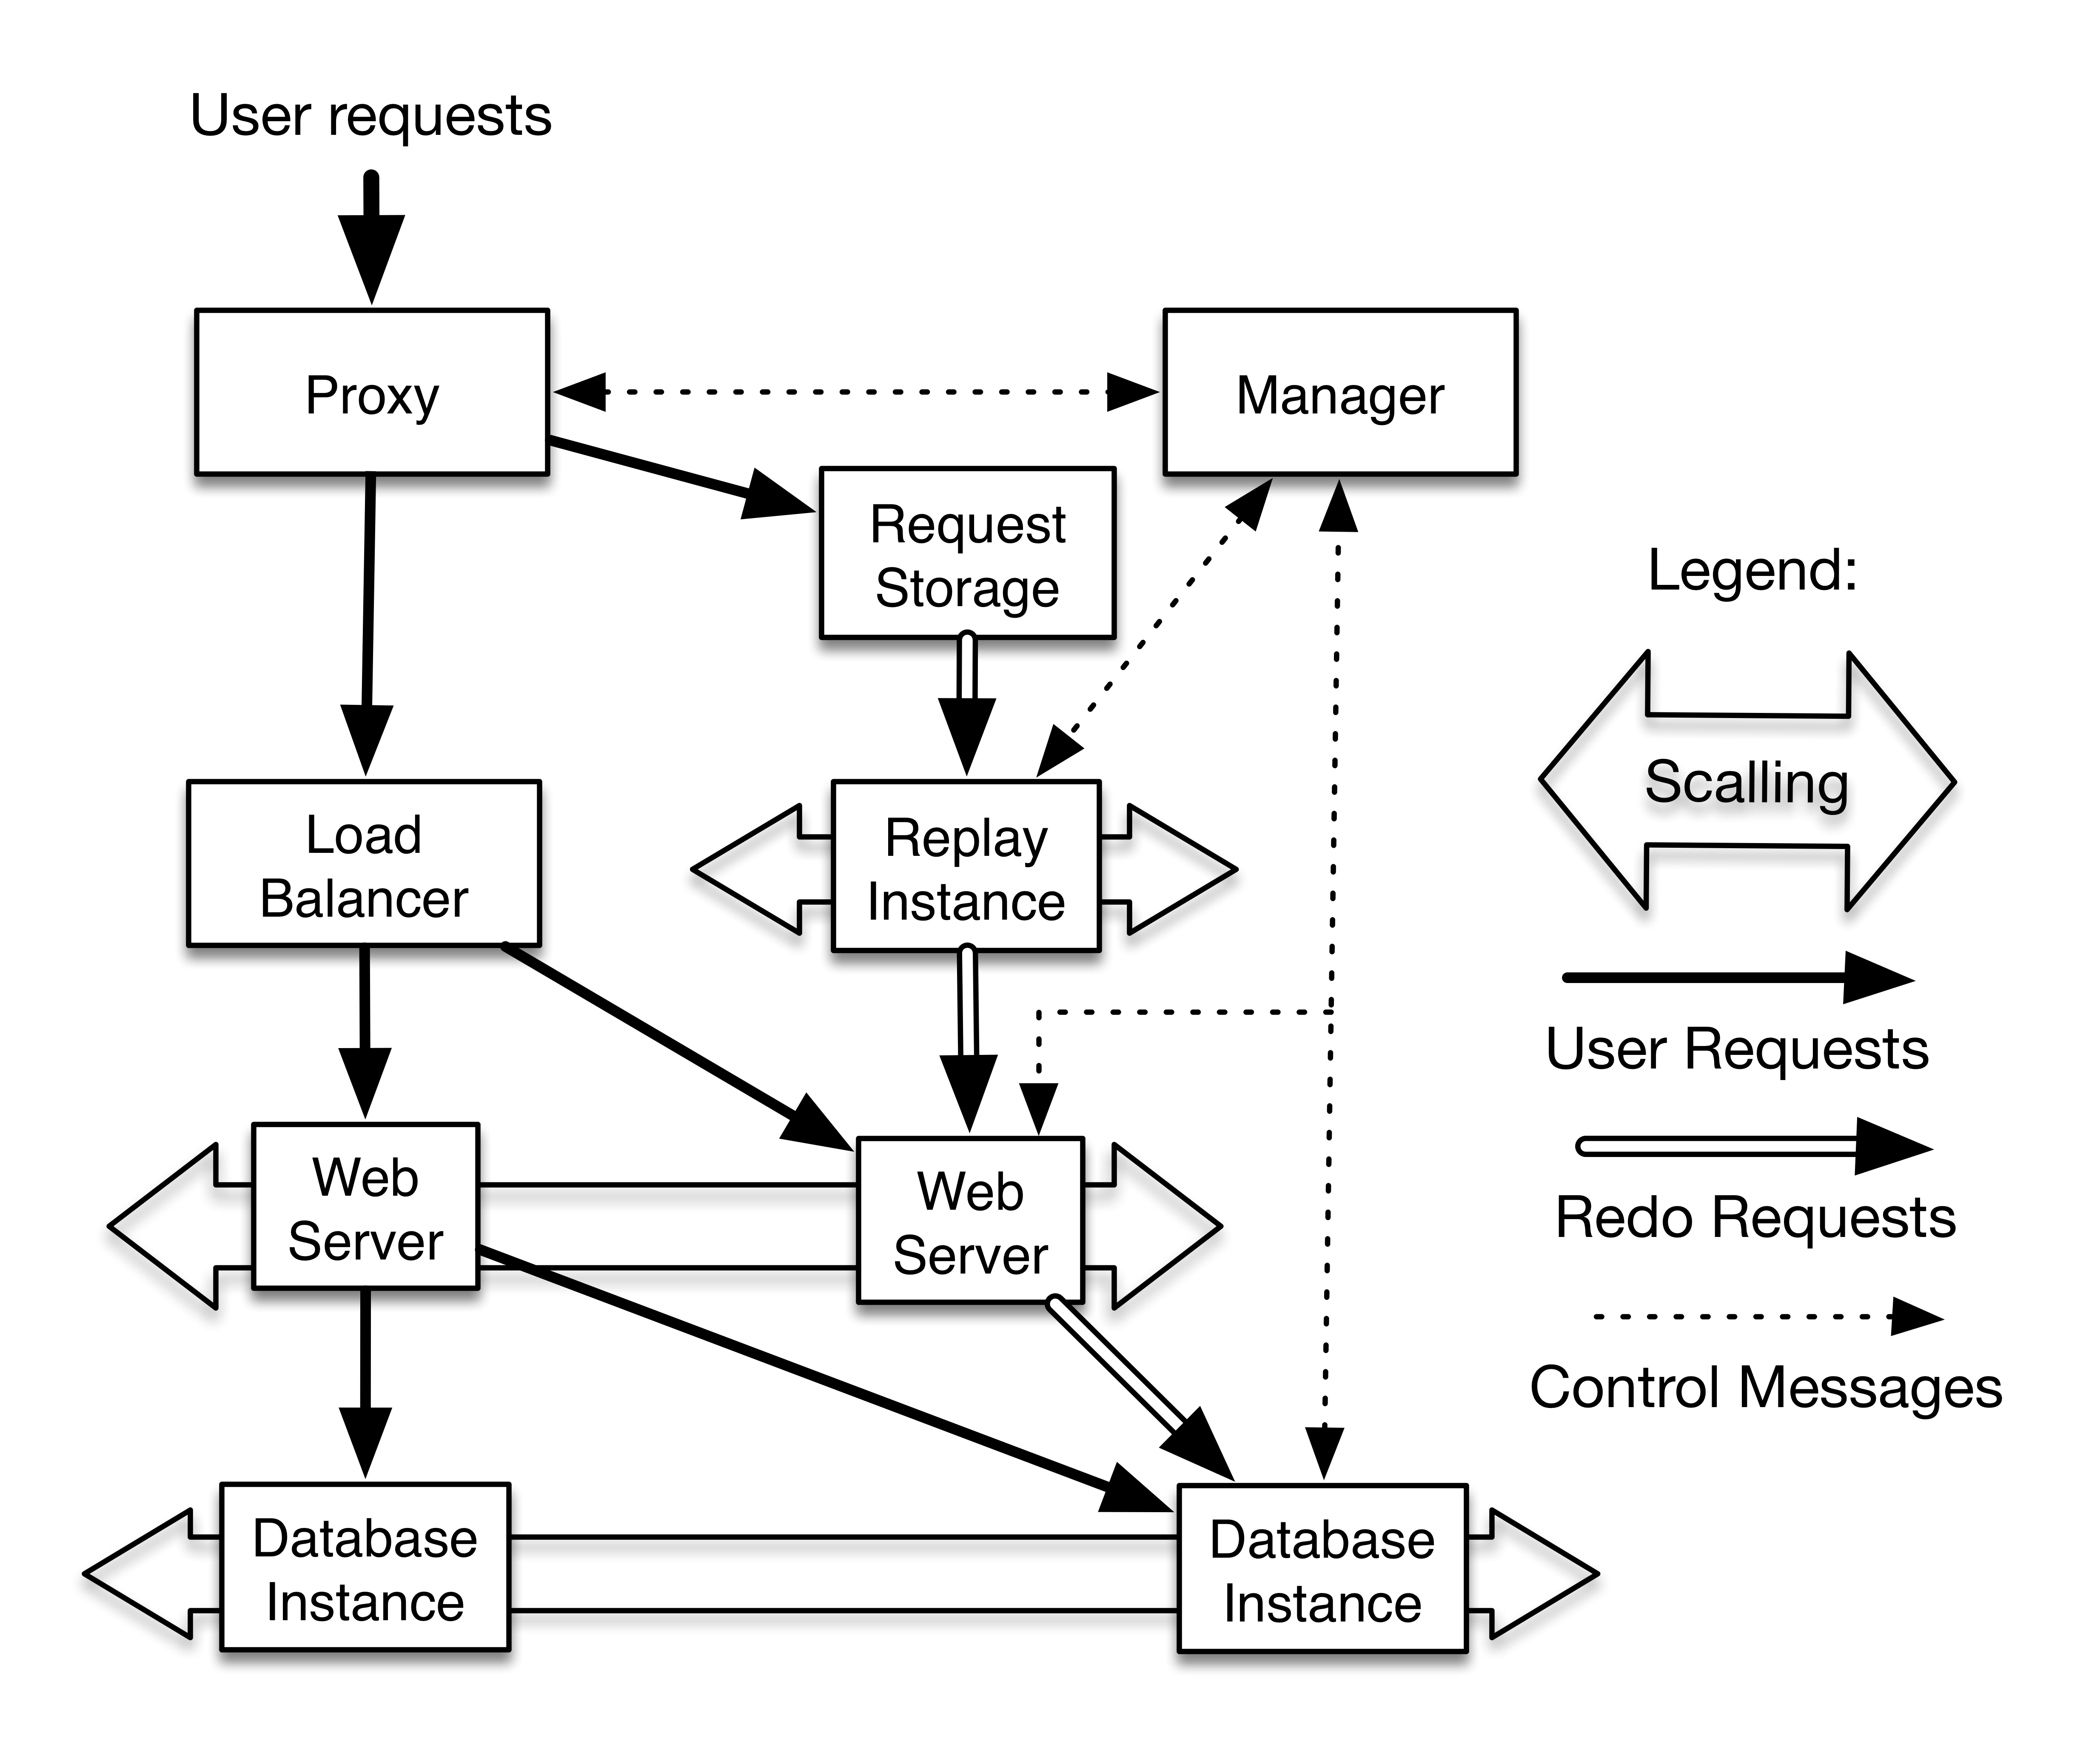
\includegraphics[width=90mm]{images/architectureTiers}
  \caption{Overview of the proposed service}
  \label{architecture}
\end{figure}

Shuttle leverages the transparency and elasticity of PaaS systems. Shuttle uses the PaaS controller to deploy an array of replay containers. Most of PaaS systems scale automatically and horizontally, i.e., they increment or decrement the number of containers based on the measurements of the containers usage. Therefore, the application-logic and data tiers scale to attend the requests from the replay containers, increasing the recovery speed. More, PaaS systems include a load balancer and nearly all deployed applications use HTTP protocol. Finally, most developers use a provided storage service, which can hide the Shuttle service.\\

%Which kind of faults? How they are detected? How they are fixed?
Shuttle recovers from software flaws faults and interaction faults from input mistakes, attacks and intrusions. To do so, Shuttle has two phases: record and replay. 

%Como e que o Shuttle vai fazer o recovery
During the record phase, the \textit{proxy} logs the user HTTP requests, adds a timestamp to its header as request id and forwards them to the load balancer. These requests are stored in an external distributed storage system using asynchronous I/O, which permits the request to proceed before the transmission has finished. After being forward by the load balancer, each request is attended by a web server. The database client auditor, deployed in each web server, logs the accessed database items. 
Each database instance has a database server auditor which intercepts the database accesses. The auditor records the client request timestamp and serializes the access to each data item, allowing multiple-reads or a single write. The access sequence of each data item is sent to the \textit{manager} to generate the dependency graph. At the end, the response is also stored in the external storage.
In summary, the external storage contains the request, response and accessed data items and the manager retrieves the accessed data items to generate the dependency graph.

%% - Replay phase
The replay phase is initialized when intrusions are detected or the application software requires an update. The detection of the fault is out of the scope of this work. In order to fix the exploited vulnerabilities, Shuttle supports software updates in the application or database instances. More, it supports the modification of user requests to remove accidental or malicious behaves. Then the \textit{manager} initiates new PaaS containers, which may include code fixes, and loads the snapshot on each database instance. The new application containers are intrusion-less because the snapshot is previous to the intrusion and the containers are renewed to include vulnerability patches. After, the requests are replayed in parallel using a set of \textit{replay containers}. The replayed requests access the database version loaded in the new containers. Since users still use the corrupted computation containers and database, the application remains online, perhaps with a degraded behavior, without exposing downtime to users. After recovery, the user requests are switched to the application with fixed state.\\


%-------------------------------------------------
The first version of Shuttle will replay every user request \cite{undoForOperators}. We assume that critical software flaws and intrusions can be detected in a short period of time, from seconds to one week. If a fault exists during a long period then the application may tolerate a longer recovery phase because the recovery process does not require application downtime. A future work may concern to perform selective replay using taint propagation via replay \cite{warp}. Still, one of the main challenges of Shuttle is to reduce the recovery time. To do so, we use two techniques: snapshot (See Section \ref{subSec:RecoveryModels}) and parallel replay.

Performing snapshots in distributed NoSQL databases (DynamoDB \cite{Decandia2007}, Bigtable \cite{Chang2008}) is not trivial since they have to be consistent with the computation tier user requests. User requests may include multiple database accesses, each of them to multiple database servers. The snapshots have to include only completed user requests. Otherwise the replay phase will be inconsistent if Shuttle replays the requests in a snapshot that contains part of the persistent state written during the previous execution of the replayed requests. Therefore, the \textit{manager} leverages the request timestamping to schedule a snapshot. The administrator defines a future instant in time, $t$, where the snapshot will occur and the manager forwards this information to every database instance. The requests, which have a timestamp bigger than $t$, write to a new version and read the latest version. The remain requests write to the previous version and read only the versions written by requests with timestamp lower than $t$. This mechanism is based on copy-on-write mechanisms.\\

To support runtime-recovery, the snapshot is loaded in a new branch, similar to the model used by git \cite{git}. The branch isolation allows multiple, perhaps simultaneous, replay attempts without compromising the exposed application behavior. More, it allows developers to test software updates with real data or discard a recovery process. To do so, the manager defines the branch used by the new user requests and by the requests which are being replayed.\\ 

Previous proposals \cite{Akkus2010} leverage the request serialization provided by snapshot isolation in relational DBMS to sort the replay operations. However, PaaS applications perform multiple \textit{transactions} accessing independent data items in NoSQL database instances. Therefore, we need a new approach to serialize the requests and the data item accesses during the replay phase. More, the data items accessed during the replay phase may change due to code updates, request modification or multi-threaded execution. While \textit{Undo for Operators} \cite{undoForOperators} uses the application protocol knowledge to establish the dependency between requests, our work aims to support any application deployed on PaaS. Therefore, we use the captured database data item access list to generate a dependency graph. The graph reflects the dependencies between requests during their execution. False dependencies in the graph do not cause data loss or inconsistent state since they are used only to order the requests replay as \textit{in} \cite{Ammann2002}.

Shuttle can not execute requests in serial order. It would not have only performance degradation but also lock the replay phase because the requests are originally executed in parallel and may depend from each other. On the other hand, PaaS applications have loosely coupled requests that share data only by data items in the database. Therefore, Shuttle will perform as many requests in parallel as possible to reduce the duration of the replay phase. The PaaS controller will auto-scale the database and application-logic tiers adding more containers. More, Shuttle manager can request the PaaS controller to initiate multiple replay containers to increase the replay performance. 
Yet, the user requests are processed in parallel using multi-threaded servers and the system messages, including the database requests, do not have a delivering order. With this in mind, Shuttle uses the access list per data item to record and to order the accesses to each data item. This method is dead-lock free if the code and requests remain equal to the original execution. Otherwise, some request may not access the same sequence of data items or read/write the same content during the replay phase creating request starvation and locking the replay process. Therefore, the database client interceptors will fetch the list of data items accessed by the original request execution and simulate the access to the remaining data items to unlock their remaining requests.\\

There are four main sources of non-determinism in each application server: concurrent threads, random number generation, time accesses and requests order. The concurrent threads are ordered using the database access mechanisms, which were introduced above. To solve the remaining issues, the \textit{proxy} adds pseudo-random number generator seed and its timestamp (also used as request ID) to the request header. Application developers can access these non-deterministic variables in a deterministic way using the PaaS middleware API. This mechanism is language independent. Despite the fact it just returns one timestamp per request, we argue that it is acceptable for most applications. \\ 

The elected database to backend the prototype is the key-value storage Voldemort \cite{Kreps}. Voldemort is an open source implementation of Amazon Dynamo DB \cite{Decandia2007} in use by Linkedin \cite{linkedin}. Key-value storage databases are common in PaaS environments because they scale properly and provide a simple put, get, delete API. We leverage the API simplicity to avoid delays and mistakes of parsing SQL queries \cite{phoenix}. More, Voldemort provides to the applications the capability of resolve the conflicts by choosing the best suited data item version. We may leverage this characteristic to solve replay conflicts and application integrity issues. \\

The external users requests and responses will be stored in the scalable NoSQL database Cassandra \cite{Lakshman2010a}. The database can be replicated to a remote site to prevent catastrophic disasters. The database server auditor can be implemented as a proxy. Shuttle uses the externally stored user requests to recover from any kind of intrusion in the computation and database instances. Since PaaS defines containers to run applications, Shuttle will collaborate with the coordinator of the PaaS system to lunch new containers using intrusion-free container images, which may include software updates. The software updates can prevent future intrusions or fix a discovered flaw \cite{Wang2011,warp}. The old containers, which may contain unknown intrusions or a corrupted operating system, are shutdown. Shuttle updates the application persistent state to be coherent with the new software version. Shuttle leverages the pay-per-usage model of PaaS to provide a cost-efficient and fast recovery service.


By replaying the user requests in parallel using intrusion-free PaaS containers and a clean database snapshot, we aim to recover from security intrusions in PaaS applications.
%!TEX encoding = UTF-8 Unicode
%- Como pensam testar a solucao e validar a vossa idea, que processo vao utilizar durante o desenvolvimento para facilitar a rrealizacao de testes e a recolha de resultados.
%- Pretendo usar um prototipo: que equipamentos/linguagens de programacao a usar
\section{Evaluation}
\label{sec:Evaluation}

The evaluation of the proposed architecture will be done experimentally, building a prototype. This evaluation aims to validate Shuttle and to prove its scalability in large implementations. The validation aims to show that Shuttle allows to recover from attacks against at least five of the OWASP Top 10 Application Security Risks: injection flaws, broken authentication, security misconfiguration, missing function level access control and using components with vulnerabilities \cite{Williams2013}. Shuttle should achieve the proposed goals and its results should match the evaluation metrics bounds which allows the Shuttle usage in real environments. We evaluate our proposal by how effective and how efficient it is, i.e., the false positive and false negative rates, the record and recovery overhead and the availability during the recovery process. In detail, we intend to measure the following:

\begin{itemize}
  \item \textbf{Recording:} We want to quantify the \textit{logging overhead} imposed measuring the \textit{delay} per request and system \textit{throughput}, \textit{resources usage} and \textit{maximum load} variance due to recording mechanisms comparing with common execution, the \textit{log size} needed to recover the system from a previous snapshot. We also will measure the time required to perform a system snapshot.
  \item \textbf{Recovery:} We aim to measure the effectiveness in terms of \textit{precision} and \textit{recall}. Precision is the fraction of the updated items that are correctly updated. Recall represents the proportion of tainted items updated out of the total number of tainted items. We can measure the number of false positives from precision, and the number of false positives from the recall. 
  We will check the recovery scalability and measure its duration for different numbers of requests, checkpoints and dependencies.
  \item \textbf{Integrity and availability:} We will measure and trace the percentage of corrupted data items and the percentage of available data items during the recovery process. These values help to define the application availability during the recovery process.
  \item \textbf{Consistent replay:} We want to guarantee that our service provides the same results as original execution if the requests and application code remain identical, even when supporting parallel and concurrent requests. 
  \item \textbf{Parallel replay:} We will measure the performance changes when the replay is performed in parallel.
  \item \textbf{Cost:} We will measure the monetary cost of the intrusion recovery process using a public cloud providers.
\end{itemize}

We will do the measurements taking into account varying sizes of the state and time between snapshots, the attack type, the damage created, the detection delay, the request arrival rate. More, we will validate if the application integrity is enough to support an adequate service during the recovery process in the hope of providing an intrusion tolerant application.

We will develop a demo web application which will be deployed on a PaaS system. Since independent user sessions would be trivial to replay, the application will have highly dependent interactions between requests from different users. The application will be a Java Spring \cite{spring} implementation of a Question and Answering (Q&A) application, like Stack Overflow \cite{stackoverflow} and Yahoo! Answers \cite{yahooAnswers}. Spring is one of the most used Java enterprise web frameworks and it is compatible with most of the current PaaS systems. To highlight the Shuttle scalability, the application will store its state in the NoSQL database Voldemort \cite{Kreps}.\\

We will develop a \emph{testing tool} to evaluate the service using HTTP requests from multiple nodes coordinated by a master node. The tool aims to simulate a real application load from multiple clients. To evaluate the efficiency, the tool will measure the response time and throughput of each user. To evaluate the effectiveness, the tool will analyze the consistency of the application responses during the recovery phase. The results will be extracted from a set of intrusion scenarios. The scenarios will include accidentally or malicious requests, external actions, e.g. ssh sessions, that compromise the PaaS containers. The scenarios will also include software updates where previous software flaws are fixed. These intrusion scenarios will be created according to typical application vulnerabilities. We will compare the overhead during normal and recovery operations. 

The prototype evaluation is branched in private cloud and public cloud. Due to public cloud costs, we will implement a test prototype on a private cloud and evaluate the final prototype on a public cloud. First, our prototype will be deployed in a PaaS system provided by AppScale \cite{Appscale} or OpenShift \cite{OpenShift}. The open source PaaS systems will run over OpenStack \cite{openstack}. Later, we will perform the final evaluation running the application over Amazon Web Service IaaS \cite{aws} or Google Cloud Platform \cite{googleCloudPlatform} to overcome our limited resources and scale to medium enterprise size scenarios.

%!TEX encoding = UTF-8 Unicode
\section{Schedule of Future Work}
\label{sec:Schedule}

Future work is scheduled as follows:
\begin{itemize}
  \item Feb 1 - Jul 30: Service implementation
  \item Jul 1 - Jul 15: Service deployment on local cloud and testing
  \item Jul 16 - Aug 1: Service deployment on public cloud (AWS), experimental evaluation of the results.
  \item April 15 - Aug 15: Write a paper describing the project
  \item Jul 15 - Set 30: Finnish the writing of the dissertation
  \item Oct 1, 2014: Deliver the MsC dissertation
\end{itemize}

The service implementation will be implemented and evaluated in phases. At the first phase, we will design the testing tool, the proxy and the demo application. At the second phase, we will handle the dependency auditors and graph. At the latest phase, we will develop the capability to perform parallel replay and integrate with a PaaS system. After, we will perform the measurements and evaluation. More details about the schedule are available in the Appendix \ref{sec:DetailedSchedule}.



%!TEX encoding = UTF-8 Unicode
\section{Conclusion}
\label{sec:Conclusion}
%Fazer o resumo do trabalho efectuado, retomando a idea, as contribuicoes definidas e a forma como estas se materializam.

Intrusion recovery services restore the system integrity when intrusions happen, instead of trying to prevent them from happening. We have presented a detailed overview of various intrusion recovery services for operating systems, databases and web applications. However, none of these projects provide a scalable service for applications deployed in multiple servers and backed by one or more databases.

Having the above in mind, we proposed Shuttle, an intrusion recovery service for PaaS, that aims to make PaaS applications operational despite intrusions. Shuttle recovers from software flaws, corrupted requests and unknown intrusions. It also supports application corrective and preventive maintenance. The major challenges are the implementation of a concurrent and consistent database snapshot, establish accurate requests dependencies, perform parallel actions replay, contain the damage spreading, repair the system state in time, avoid application downtime and keep the application source code unmodified as much as possible.

Shuttle removes the intrusion effects in PaaS applications and restores the application to a correct state recreating an intrusion-free state. We propose, to the best of our knowledge, the first intrusion recovery service for PaaS with support to NoSQL databases.
 

\vspace{8mm}

\textbf{Acknowledgments} We are grateful to Professor Miguel Pupo Correia for the discussion and comments during the preparation of this report. This work was partially supported by Fundação para a Ciência e Tecnologia (FCT) via INESC-ID annual funding through the RC-Clouds - Resilient Computing in Clouds - Program fund grant (PTDC/EIA-EIA/115211/2009).
\clearpage
%!TEX encoding = UTF-8 Unicode
\newgeometry{left=3cm,top=1.5cm}
\begin{sidewaysfigure}
  \appendix
\section{Detailed Schedule}
\label{sec:DetailedSchedule}
  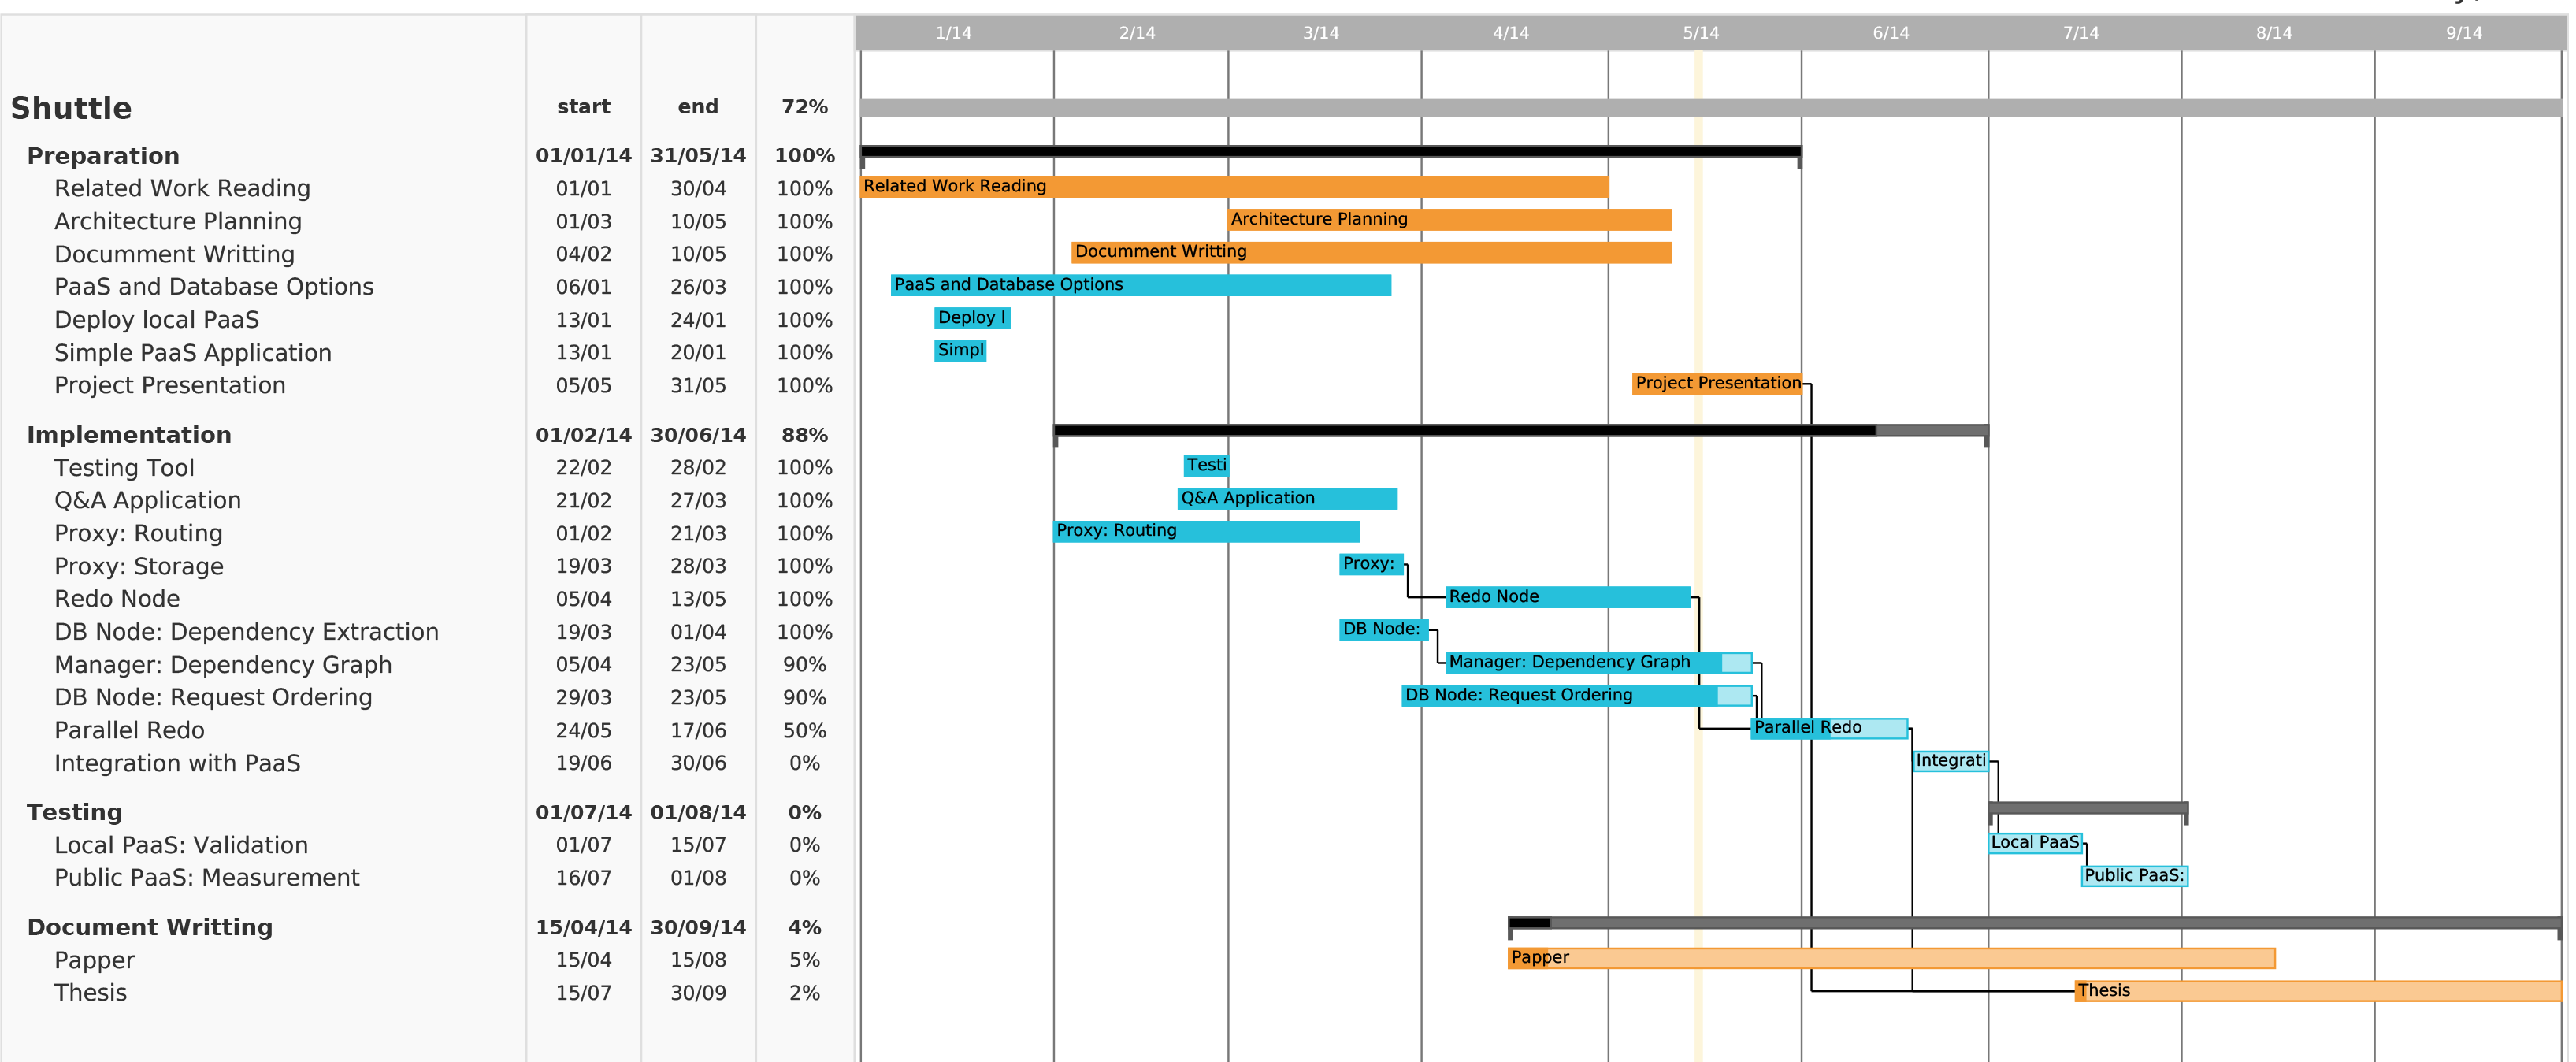
\includegraphics[width=220mm]{images/gantt}
  \caption{Project Gantt Schedule}
  \label{gantt}
\end{sidewaysfigure}
\restoregeometry

\clearpage
\bibliographystyle{IEEEtran}
\bibliography{./references/manual,./references/All}

\end{document}
